\part{Hybrid Switched Capacitor LED driver}
\chapter{Hybrid Switched Capacitor Converter}
\label{ch:H-SCC}
Driving high power LEDs using a switched capacitor converter challenges the operation of these converters. The SCC provides good performance in voltage-to-voltage conversion, but it can not directly provide regulated current. In low power applications, that is solved by using a linear regulator in series with the LED string, however that is not a valid solution for general lighting where high power and high current are needed. Combining switched capacitors with inductors can provide efficient converters for LED lighting, where the use of inductors provide a tight and efficient regulation, and the use of a switched capacitor allows to reduce the voltage stress in the components, in turn reducing switching losses and the volume of the inductor.

The \emph{hybrid} switched capacitor converter (H-SCC) is a merge of a switched capacitor and an inductive converter, which will be introduced in this chapter. The first section introduces the basic knowledge about switched capacitor converters (SCC) to understand the enhancements, modifications and characteristics of the \emph{hybrid}-SCC. The second section presents the H-SCC topology and  operation. The third section introduces LED drivers circuits based on H-SCC, being them the fundamental circuits of this disoperation. Additionally, different driver architectures are described in this section giving a broader perspective of different applications of H-SCC in LED drivers.


\section{State of the Art}
In  commercial ICs but also in research the integration and miniaturization characteristics of Switched Capacitor Converters (SCCs) have an application for LED drivers. Commercially there is a large portfolio of available integrated circuits (ICs) ( designated as Charge-Pumps (CPs))  for backlighting in portable devices, \emph{i.e.}  \emph{MAX8930} \footnote{Maxim\textsuperscript{\textregistered} WLED Charge Pump, RGB, OLED Boost, LDOs with ALC and CAI }, \emph{MCP1252/3} \footnote{Microchip\textsuperscript{\textregistered} Low noise, Positive-Regulated Charge Pump}. These circuits can drive White or RGB LEDs from a Lithium-Ion battery by merely adding a few external capacitors,  as shown in the block diagram of Figure~\ref{fig:SCC_backlight_LED}. Generally these chips integrate a SCC with different conversion ratios, along with a linear regulator for each channel. Various publications ~\cite{07Feng,09Wu,10Yin} proposed different modifications of the architectures in order to reduce the parasitic losses, bringing the efficiency close to the theoretical limit. The power ratings in these drivers are below 1$W$ at currents below hundred mili-Amperes with efficiencies between 70\%-90\% depending on the operation point.

\begin{figure}[!ht]
    \centering
    \begin{circuitikz} [american voltages,scale=0.65]
    \ctikzset{bipoles/length=1cm}
   \draw[thick] (2.5,0.25) --
                (2.5,6.5) --
                (11.5,6.5) --
                (11.5,0.25) --
                (2.5,0.25);

    %Draw SCC block with capacitors
    \draw (3,1) --
          (3,6) --
          (5,6) --
          (5,1) --
          (3,1);

    \draw (4,3) node[rotate=90,anchor=west] {SCC};

    \draw (5,5.5) to[short,-o] (14,5.5);
    \draw (13,5.5) to[capacitor] (13,4.5) node[sground]{};

    \draw (4,1) -- (4,0) node[sground,scale=0.75]{};

   %Draw linear drivers
   \draw  (4,0.5) -- (10.5,0.5) -- (10.5,1);

   %First transitor
   \draw   (10,1) -- (10,1.5) node[npn,anchor=E,scale=0.5](npn1){}
           (npn1.C) -- (10,2.75) to[short,-o] (12,2.75);

   %Second transitor
   \draw  (10,1) -- (11,1)
           node[npn,anchor=E,scale=0.5](npn2){}
           (npn2.C) -- (11,2.25) to[short,-o] (12,2.25);

   %Controller box
   \draw (5.5,1) -- (8.5,1) -- (8.5,3) -- (5.5,3) -- (5.5,1);
   \draw (5.75,2) node[anchor=west, text width = 1.75cm]{Intensity Controller};
   \draw (npn2.B) -| (8.5,2);
   \draw (npn1.B) -| (8.5,2);

   %LEDs

   \draw (14,5.5) to[short,o-] (15,5.5)
                    to[leD*] (15,2.75) to[short,-o] (12,2.75);

   \draw (15,5.5) -- (17,5.5)
                    to[leD*] (17,2.25) to[short,-o] (12,2.25);

   %Add battery

   \draw (-1,0) node[sground,scale=0.75]{} to[battery = $v_{src}$] (-1,5.5)
         -- (3,5.5);

   \draw (3,5) -- (1.5,5) to[C,l_=$c_2$] (1.5,3.5) -- (3,3.5);
   \draw (3,3) -- (1.5,3) to[C,l_=$c_1$] (1.5,1.5) -- (3,1.5);


    \end{circuitikz}
    \caption{Block diagram of the common architecture used in \emph{charge pump} LED drivers for small screens backlighting in portable applications.}
    \label{fig:SCC_backlight_LED}
\end{figure}

With respect to general lighting there are a few research publications that report the use of SCCs. In 2008, ~\citeauthor{08Lee}~\cite{08Lee} presented a step-down converter supplied from rectified 220$V_{rms}$ providing 15W with a 95\% peak efficiency. The proposed architecture directly supplied the LED string from the capacitors, controlling the output power by changing the switching frequency.

In 2012, ~\citeauthor{2012Kline}~\cite{2012Kline} proposed a isolated converter that combined a SCC stage with series-LC resonant converter delivering 15.5W with an efficiency of  92\%.  The SCC stage decreased  the rectified mains voltage, reducing the voltage stress in switches, capacitors and the elements of the resonant tank, allowing to diminish  the volume of the passive components and the total silicon area. The LED current is regulated by modulating frequency and duty cycle.  The architecture was recently implemented in modular silicon dies, that can be stacked in order to adjust to different mains voltages~\cite{2013Kline}.


%different LED driver architectures will be presented along with architecture and control modifications that extends the range of operation of the converter.

\section{Switched Capacitor Converter}

SCCs are a family of SMPS circuits that provide power conversion using only switches and capacitors. % as shown in Figure~\ref{fig:demo_full_sch}.
A SCC has two or more operation modes, referred as phases, and each operating mode is associated with a different circuit arrangement of the capacitors. The SCC is sequentially switching between the different modes, providing a voltage conversion between input and output. The circuit in Figure~\ref{fig:demo_full_sch} is a two phase 3:1 Dickson that provides a step down conversion ratio of $\frac{1}{3}$. During the first phase the odd switches are closed, resulting in the circuit of Figure~\ref{fig:demo_full_p1}. During the second phase, the even switches are closed, resulting in the circuit of Figure~\ref{fig:demo_full_p2}.

Dickson and Ladder are the preferred SCC topologies used in this dissertation. Both topologies have been selected since they share a similar characteristics that favour the design of H-SCCs: Equal voltage ripple among all \emph{pwm}-nodes. Despite that in the following examples are based on a Dickson or a Ladder  converter, they hold for any other well posed SCC topology~\cite{Seeman:EECS-2009-78}.

\begin{figure}[!h]
\centering
\ctikzset { bipoles/length=1cm}
%\ctikzset { scale=0.5}
    \begin{subfigure}[t]{\textwidth}
    %\floatbox[{\capbeside\thisfloatsetup{capbesideposition={left,top},capbesidewidth=1cm}}]{figure}[\FBwidth]
%{\caption{A test figure with its caption side by side}\label{fig:test}}{
    \centering
    %\ctikzset { bipoles/length=1cm}
        \begin{circuitikz}[american voltages,scale=0.6]
        %\draw (0,11) node[anchor=north]{ };
        \draw
                %Input Supply
                (0,0)  to[V=$v_{i}$]
                %Draw Switches
                (0,10)  --
                (5,10)  to[switch=$s_1$] %S1
                (5,8)   to[switch=$s_2$] %S2
                (5,6)   to[switch=$s_3$] %S3
                (5,4) --
                %left branch
                (3,4)   to[switch=$s_7$]
                (3,2)   to[switch=$s_6$]
                (3,0);

        \draw   %right branch
                (5,4) --
                (7,4)   to[switch=$s_4$]
                (7,2)   to[switch=$s_5$]
                (7,0) -- (0,0);

        \draw %Capacitor C1
               (3,2) -- (2,2) -- (2,4)
                to[pC=$c_1$] (2,8) --
               (5,8);

        \draw %Capacitor C2
                (7,2) -- (8.25,2) --
               (8.25,4) to[pC=$c_2$](8.25,6) --
               (5,6);

        \draw %Capacitor C3
               (5,0) to[pC=$c_3$,-*]
               (5,4);

        \draw (7,4) --([hs]8.25,4 |- 7,4) arc(180:0:\radius) to[short,-o] (10,4) to[open,v^=$v_{out}$] (10,0)
        (7,0) to[short,-o] (10,0) node[anchor=west] {};
    \end{circuitikz}

     \subcaption{3:1 Dickson Converter.}
     \label{fig:demo_full_sch}
    \end{subfigure}

    \begin{subfigure}[t]{\textwidth}
    \centering
    %\ctikzset { bipoles/length=1cm}
        \begin{circuitikz}[american voltages,scale=0.6]
        \draw (-1,7) node[anchor=north]{ };
        \draw
                %Input Supply
                (-1,0)  to[V=$v_{i}$]
                %Draw Switches
                (-1,6)  --
                (4,6);

        %Capacitor C1
        \draw   (4,3) to[pC=$c_1$] (4,6);

        %Capacitor C2
        \draw (2,0)to[pC=$c_2$](2,3) --(4,3);

        %Capacitor C3
        \draw  (-1,0)--
               (6,0) to[pC=$c_3$]
               (6,3) -- (4,3);

         \draw (6,3) to[short,-o] (7.5,3) node[anchor=west] {};
         \draw (6,0) to[short,-o] (7.5,0) node[anchor=west] {};
         \draw (7.5,3) to[open,v^=$v_{out}$] (7.5,0);
         \end{circuitikz}
     \subcaption{First phase, odd switched are closed and even switches are open.}
     \label{fig:demo_full_p1}
     \end{subfigure}

     \begin{subfigure}[t]{\textwidth}
      \centering
      \begin{circuitikz}[american voltages,scale=0.6]
        \draw (0,7) node[anchor=north]{ };
        \draw   %Input Supply
                (-1,0)  to[V=$v_{i}$]
                %Draw Switches
                (-1,6);

        \draw   (5,3) to[pC=$c_2$] (5,6);

        \draw %Capacitor C1
               (2,0)to[pC=$c_1$](2,6) --(5,6);

        \draw %Capacitor C3
               (5,0) to[pC=$c_3$]
               (5,3) -- (5,3);

         \draw (5,3) to[short,-o] (7.5,3) node[anchor=west] {};
         \draw (-1,0) to[short,-o] (7.5,0) node[anchor=west] {};
         \draw (7.5,3) to[open,v^=$v_{out}$] (7.5,0);

         %\draw ()
         \end{circuitikz}
     \subcaption{Second phase, even switched are closed and odd switches are open.}
     \label{fig:demo_full_p2}
     \end{subfigure}
\caption{}
\label{fig:emo_full}
\end{figure}

\subsection{Conversion ratio}
\label{ch:conversion_ratio}
The conversion ratio of the converter and the steady state voltages in the capacitors are obtained applying Kirchhoff's voltage law (KVL) for each circuit mode, and combining the different linear independent equations.

KVL equations of the first phase are:
\begin{align}
\label{eqn:ph1_kvl}
\begin{split}
  v_{src} - v_{c_1} - v_{c_2} &=0, \\
  v_{out} - v_{c_2}  &=0,\\
  v_{out} - v_{c_3}  &=0.
\end{split}
\end{align}

KVL equations of the second phase are:
\begin{align}
\label{eqn:ph2_kvl}
\begin{split}
  v_{c_1} - v_{c_2} - v_{c_3} &=0, \\
  v_{out} - v_{c_3}  &=0.
\end{split}
\end{align}

Selecting the linear independent equations from eq.(\ref{eqn:ph1_kvl}) and eq.(\ref{eqn:ph2_kvl}), a solvable system can be formulated as
\begin{align}
\label{eqn:sys_kvl}
\begin{split}
  v_{src} - v_{c_1} - v_{c_2} &=0, \\
  v_{c_1} - v_{c_2} - v_{c_3} &=0, \\
  v_{out} - v_{c_2}  &=0,\\
  v_{out} - v_{c_3}  &=0,
\end{split}
\end{align}
solving it yields to
\begin{align}
\label{eqn:sol_kvl}
\begin{split}
  v_{out} =  v_{c_3} = v_{c_2} &=\frac{V_{src}}{3} , \\
  v_{c_1} &=\frac{2 \cdot V_{src}}{3} ,
\end{split}
\end{align}
hence the converter conversion ratio is

\begin{equation}
\label{eqn:m_kvl}
m_i = \frac{v_{out}}{v_{src}} = \frac{1}{3}.
\end{equation}

This result shows that the conversion ratio is defined by the topology of the converter and independent of the switching operating regime. From now on, the conversion ratio defined by the topology will be referred as the \emph{intrinsic} conversion ratio and defined as $m_i$.

\subsection{Output voltage regulation}

A SCC has a fixed conversion ratio only defined by its topology and not by its operation regime. The conversion ratio of the converter can not be adjusted changing frequency or pulse width as in the case of inductive based converters, therefore the converter can not directly provide voltage regulation.


\begin{SCfigure}
\centering
\caption{Linear regulated switched capacitor}
\label{fig:linear_scc}
\ctikzset { bipoles/length=1cm}
\tikzstyle{block} = [draw, rectangle, fill=white!40]

\begin{circuitikz} [american voltages, scale=0.65]
\draw   (-3,0) --
        (-4,0) to[V = $v_{src}$]
        (-4,3) -- (-3,3);

 \draw  (0.5,3) to[open,v^=$m \cdot v_{src} $] (0.5,0);

 \draw  (0,3) -- (1,3) to[generic,v^=$v_{drop}$,i_=$i_o$]
        (5,3) -- (6,3) to[R,l_=$load$,v^=$v_{o}$]
        (6,0) -- (0,0);

 \node [block] (SCC) [minimum height = 2.6cm, minimum width = 1.95cm] at(-1.5,1.5) {SCC};
 %\node [block] (SCC) [minimum height = 4pt, minimum width = 3pt] at(-.5,1.5) {SCC};
\end{circuitikz}
\end{SCfigure}

Indirectly, there is always the possibility to regulate the output voltage by means of a linear regulator, thus the output voltage is adjusted by drooping the excess voltage ($v_{drop}$) in a series element with the load, as shown in the schematic of Figure~\ref{fig:linear_scc}. This can be achieved in two ways: Using an external liner regulator connected  between the converter output and the load, or what is more common, using or \emph{'misusing'}  the behaviour of the SCC in order to provide this linear regulation characteristic~\cite{Ng:EECS-2011-94} . Regulating the load in such a way reduces the efficiency of the converter.%in fact the converter's efficiency decreases as the difference between $m \cdot v_{src}$ and $v_o$ increases. Actually,
 Like a linear regulator,  the efficiency of the converter can be written as function of $v_{src}$ and $v_o$ as
\begin{equation}
\eta = \frac{P_o}{P_i} = \frac{v_o \cdot i_o}{m \cdot v_{src} \cdot i_o} = \frac{v_o}{m \cdot v_{src}}.
\label{eq:eff_vo}
\end{equation}

Figure~\ref{fig:eff_crv_linear_vs_scc_linear} plots the theoretical maximum efficiency with respect of the effective conversion ratio of the power converter  $m_e = v_o/v_{src}$. Comparing the characteristics of a single linear regulator and a linear regulated 2:1 SCC shows that for conversion ratios below $1/2$ the SCC converter has better efficiency, however above $1/2$ the SCC is not longer operative.

\begin{SCfigure}
\centering
\begin{circuitikz}
    \begin{scope}%[xshift = 8cm, yshift=0cm]
        \draw[->] (0,0) -- (4,0) node[anchor=south] {$  m_e $};
        \draw[->] (0,0) -- (0,4) node[anchor=east] {$\eta $};

        %Ticks X
        \draw (3,2pt) -- (3,-5pt)  node[anchor=north west] {$1$};
        \draw (1.5,2pt) -- (1.5,-5pt)   node[anchor=north west] {$\frac{1}{2}$};

        %Ticks Y
        \draw (2pt,3) -- (-5pt,3) node[anchor=east] {$100\%$};
        \draw (2pt,1.5) -- (-5pt,1.5) node[anchor=east] {$50\%$};

        %Markers
        \draw[dotted] (3,3) -- (3,0);
        \draw[dotted] (3,3) -- (0,3);
        \draw[dotted] (1.5,3) -- (1.5,0);
        \draw[dotted] (1.5,1.5) -- (0,1.5);


        \draw[thick,dashed] (3,3) -- (0,0);
        \draw[thick] (1.5,3) -- (0,0);
\end{scope}
\end{circuitikz}
\caption{Maximum theoretical efficiency plotted as function of the conversion ratio: \emph{dashed line} - linear regulator ; \emph{thick line} - 2:1 linear regulated SCC}
\label{fig:eff_crv_linear_vs_scc_linear}
\end{SCfigure}

\subsection{Multiple conversion ratio converters}

Multiple conversion ratio converters enable to extend the regulation margins and increase the conversion efficiency. Figure~\ref{fig:eff_crv_linear_vs_scc_linear} shows the limitations of a 2:1 SCC. First, the converter is only operative for conversion rations below $1/2$. Second, as the conversion ratio moves below the intrinsic conversion  ratio of the converter ($1/2$) the efficiency linearly decreases.
Other topologies, like the one of Figure~\ref{fig:M_SCC_ckt}, have multiple conversion ratios - $\frac{1}{3}$, $\frac{1}{2}$, $\frac{2}{3}$ and $1$ - that extend the operation margins and increase the efficiency of the converter as shown in the plot of Figure~\ref{fig:M_SCC_plt}. A detailed analysis of this converter is presented in the appendicle X, section B.

\begin{figure}[!h]
\centering
\ctikzset { bipoles/length=1cm}
\begin{subfigure}[t]{.95\textwidth}
    \centering
    %\raggedleft
    \begin{circuitikz} [american voltages,scale=0.65]
    \draw (0,7) node[anchor=south] {};
    \draw
        (-1.5,0) node[sground] {} to[V = $v_{src}$]
        (-1.5,3) -- (0,3) to[switch=$s_1$]
        (2.5,3) to[capacitor=${c_1}$]
        (3.5,3) -- (5,3) to[switch=$s_2$]
        (6.5,3) to[short]
        (7,3);

    %Switch s9
    \draw (4,3) -- (4,1.5) to[switch=$s_9$] (2,1.5) -- (2,-2);

    %Switch s4
    \draw (5,3)  to[switch=$s_4$] (5,1) node[sground] {} ;

    %Switch branch to load
    \draw (2,3) --
          (2,4.5) to[switch=$s_3$]
          (7,4.5) to[short,-*]
          (7,3) -- (7,-2);

    \draw (0,3) -- (0,-2) to[switch=$s_5$] (2,-2) -- (2.5,-2) to[capacitor=${c_2}$] (3.5,-2) -- (5,-2) to[switch=$s_6$] (6.5,-2) -- (7,-2);

    %Switch s7
    \draw (2,-0.5) to[switch,l_=$s_7$] (7,-0.5);

    %Switch s8
    \draw (4,-2)  to[switch=$s_8$] (4,-4) node[sground] {} ;


    %Load and capacitor C2
    \draw (8,0) node[sground]{} to[capacitor,l_=$c_o$] (8,3);

    \draw (7,3) to[short,-o] (9,3) node[anchor=west] {$v_o$};

    \end{circuitikz}
    \caption{Multiple conversion ratio SCC.}
    \label{fig:M_SCC_ckt}
\end{subfigure}

\begin{subfigure}[t]{.95\textwidth}
    \centering
    %\raggedright
    \begin{circuitikz}
        \begin{scope}[xscale=0.9, yscale=0.85]
        \draw (0,4.5) node[anchor=south] {};
        \draw[->] (0,0) -- (7,0) node[anchor=south] {$  m_e $};
        \draw[->] (0,0) -- (0,4) node[anchor=east] {$\eta $};

        %Ticks X
        \draw (6,2pt) -- (6,-5pt)  node[anchor=north  ] {$1$};
        \draw (3,2pt) -- (3,-5pt)   node[anchor=north ] {$\frac{1}{2}$};
        \draw (4,2pt) -- (4,-5pt)   node[anchor=north ] {$\frac{2}{3}$};
        \draw (2,2pt) -- (2,-5pt)   node[anchor=north ] {$\frac{1}{3}$};
        \draw (0,0) node[anchor=north east] {$0$};

        %Ticks Y
        \draw (2pt,3) -- (-5pt,3) node[anchor=east] {$100\%$};
        \draw (2pt,1.5) -- (-5pt,1.5) node[anchor=east] {$50\%$};

        %Markers
        \draw[dotted] (6,3) -- (6,0);
        \draw[dotted] (6,3) -- (0,3);
        \draw[dotted] (3,3) -- (3,0);
        \draw[dotted] (3,1.5) -- (0,1.5);


        \draw[thick,dashed] (6,3) -- (0,0);
        \draw[thick] (0,0)--(2,3)--(2,2) -- (3,3) -- (3,2.25) -- (4,3) -- (4,2) -- (6,3);
    \end{scope}
\end{circuitikz}
\caption{Maximum theoretical efficiency plotted as function of the conversion ratio: \emph{dashed line} - Single linear regulator; \emph{thick line} - Linear regulated multiple conversion ratio SCC.}
\label{fig:M_SCC_plt}
\end{subfigure}

\caption{}
\label{fig:eff_crv_linear_vs_mult_scc_linear}
\end{figure}


\subsection{Converter output nodes}

The previous section presented switched capacitor converters with the load connected to a node that provides a fixed conversion ratio. Actually, that is the most common way of employing these converters, however a SCC can supply the load from other nodes. Two types of nodes can be identified in a Switched Capacitor Converter: Fixed voltage \emph{dc}-nodes, node $a$ in Figure~\ref{fig:dc_pwm_nodes}, and floating voltage \emph{pulse width modulated} nodes (\emph{pwm}-nodes),  node $b$ in Figure~\ref{fig:dc_pwm_nodes}.

\begin{figure}[!h]
\centering
\ctikzset { bipoles/length=1cm}
\begin{circuitikz}[american voltages,scale=0.65]
\draw
        %Draw Switches
        (0,0)  to[V=$v_{src}$]
        (0,8)  --
        (5,8)   to[switch=$s_1$,-*]
        (5,6)   to[switch=$s_2$]
        (5,4)   to[switch=$s_3$]
        (5,2)   to[switch=$s_4$]
        (5,0)  --
        (0,0)

        (5,6) to[short,-o]
        (8,6) node[anchor=west] {$b \rightarrow$  \emph{pwm}  node}

        (5,4) to[short,-o]
        (8,4) node[anchor=west] {$a \rightarrow$ \emph{dc} node}

%Draw Capacitors
        (5,2) --
        (3,2) to[C=$c_{fly}$]
        (3,6)--
        (5,6)

        (5,0) --
        (7,0) to[C=$c_{dc}$,mirror]
        (7,4)--
        (5,4);

  \begin{scope}[xshift=13cm,yshift=0.2cm]
  \draw [->] (-0.1,0) -- (5,0) node[anchor=west]{$t$};
  \draw [->] (0,-0.1) -- (0,2.5) node[anchor=east]{$v_a$};
  %\draw (0,-1) node[anchor=south]{0}
%        (1.25,-1) node[anchor=south] {$T$}
%        (2.5,-1)  node[anchor=south] {$2T$}
%        (3.75,-1) node[anchor=south] {$3T$} ;

  \draw [thick] (0,1) -- (0.75,0.75) -- (0.75,0.95) -- (1.25,0.80)
                      -- (1.25,1)-- (2,0.75) -- (2,0.95) -- (2.5,0.80)
                      -- (2.5,1)-- (3.25,0.75) -- (3.25,0.95) -- (3.75,0.80);

  \draw [dashed] (0,0.875) -- (4,0.875) node[anchor=west]{$v_a$} ;
  \end{scope}

  \begin{scope}[xshift=13cm,yshift=4 cm]
  \draw [->] (-0.1,0) -- (5,0) node[anchor=west]{$t$};
  \draw [->] (0,-0.1) -- (0,2.5) node[anchor=east]{$v_b$};
  %\draw (0,-1) node[anchor=south]{0}
%        (1.25,-1) node[anchor=south] {$T$}
%        (2.5,-1)  node[anchor=south] {$2T$}
%        (3.75,-1) node[anchor=south] {$3T$} ;

  \draw [thick] (0,2) -- (0.75,1.85) -- (0.75,1) -- (1.25,0.80) --
                (1.25,2) -- (2,1.85) -- (2,1) -- (2.5,0.80) --
                (2.5,2)-- (3.25,1.85) -- (3.25,1) -- (3.75,0.80);

  \draw [dashed] (0,1.515) -- (4,1.515) node[anchor=west]{$v_b$} ;
  \end{scope}

\end{circuitikz}
\caption {Node types in a 2:1 converter: Node $a$ is a \emph{dc}-node; its voltage, $v_a$ is plotted in the bottom graph. Node $b$ is a \emph{pwm}-node; its voltage, $v_b$, is plotted in the top graph.}
\label{fig:dc_pwm_nodes}
\end{figure}

Fixed voltage \emph{dc}-nodes are the common output nodes of a SCC. A \emph{dc}-node supplies the load with a fixed conversion ratio defined by the topology, and  with a low voltage ripple thanks to the capacitor in parallel with the load. The capacitors that are connected between a \emph{dc}-node and ground are  \emph{dc}-capacitors as shown in the Fig. \ref{fig:dc_pwm_nodes}. A SCC can have one or more \emph{dc}-capacitors, however topologies with a reduced number of these trend to have a better area utilization, since these \emph{dc}-capacitors do not contribute to the charge transportation~\cite{Seeman:EECS-2009-78}.

Floating \emph{pulse width modulated}-nodes (\emph{pwm}-nodes) have been rarely used as outputs until a couple of recent publications~\cite{2012Kumar, 2012Kline} presented the advantages of using them. \emph{pwm}-nodes have been normally considered  internal to the converter without any added functionality, but actually the conversion possibilities of SCCs can be further enhnaced by using these nodes as outputs.
\emph{pwm}-nodes are accessible from the terminals of flying capacitors ($c_{fly}$), delivering a floating pulse-width-modulated (PWM) voltage with an added \emph{dc} offset of a fraction of the input voltage with respect to ground. The magnitudes are related to the SCC topology. The pulsating voltages can be filtered using an inductive-capacitive filter (\emph{LC}), allowing to supply a \emph{dc} load with the averaged voltage of the node. Furthermore the \emph{pwm} voltage at the node can be controlled by adjusting the duty
cycle of the SCC, enhancing the regulation capabilities of these outputs compared to the fixed value of the \emph{dc}-nodes.

\section{Hybrid-Switched Capacitor Converter}
A Hybrid Switched Capacitor Converter (H-SCC) uses a low pass filter to supply a \emph{dc} voltage from a \emph{pwm}-node, as shown in Figure~\ref{fig:3_1_hscc}. The low pass filter is composed of an inductor $l_o$ and capacitor $c_o$, and averages the \emph{pwm}-voltage of the switching node $v_x$.

\begin{figure}[t]
\ctikzset { bipoles/length=1cm}
\centering
    \begin{circuitikz}[american voltages,scale=0.6]

    \draw
            %Input Supply
            (-1,0)  to[V=$v_{src}$]
            %Draw Switches
            (-1,10)  --
            (5,10)  to[switch=$s_1$] %S1
            (5,8)   to[switch=$s_2$] %S2
            (5,6)   to[switch=$s_3$] %S3
            (5,4) --
            %left branch
            (3,4)   to[switch=$s_7$]
            (3,2)   to[switch=$s_6$]
            (3,0);

    \draw   %right branch
            (5,4) --
            (7,4)   to[switch,l_=$s_4$]
            (7,2)   to[switch,l_=$s_5$]
            (7,0) -- (-1,0);

    % Nodes
    \draw   (5,8) node[anchor=west] {$n_1$};
    \draw   (5,6) node[anchor=east] {$n_2$};
    \draw   (2,2) node[anchor=east] {$n_3$};
    \draw   (8.25,2) node[anchor=west] {$n_4$};



    \draw %Capacitor C1
           (3,2) -- (2,2)
            to[pC,l_=$c_1$] (2,8) --
           (5,8);

    \draw %Capacitor C2
           (7,2) --
           (8.25,2)  to[pC,l_=$c_2$](8.25,6) --
           (5,6);

    \draw  %Inductor
            (8.25,6) to[L=$l_o$,-o] (12,6);


    \draw %Capacitor C3
           (5,0) to[pC,l_=$c_3$,-*] (5,4) node[anchor=south east] {$n_{dc}$};

     %\draw (7,4) to[short,-o] (10,4) node[anchor=west] {};
     \draw (7,0) to[short,-o] (12,0) node[anchor=west] {};
     \draw (12,6) to[open,v^=$v_{out}$] (12,0);
     \draw (8.25,6) node[anchor=south] {$v_x$};

     \draw (11.5,0) to[pC,l=$c_{o}$] (11.5,6);

     \end{circuitikz}
 \caption{ H-SCC with a 3:1 Dickson topology with the inductor connected to the second \emph{pwm}-node.}
 \label{fig:3_1_hscc}
\end{figure}

\begin{SCfigure}
\centering
\begin{circuitikz}[american voltages,xscale=0.55,yscale=0.65]
\begin{scope}
  \draw [->] (0,0) -- (10,0) node[anchor=west]{$t$};
  \draw [->] (0,0) -- (0,5.5) node[anchor=east]{$v_x$};

  %Vertical ticks
  \draw (2pt,4) -- (-5pt,4) node[anchor=east]  {$v_{src} \frac{2}{3}$};
  \draw (2pt,2.5) -- (-5pt,2.5) node[anchor=east]  {$v_{src} \frac{1}{3}$};

  %Horizontal ticks
  \draw (1.25,2pt) -- (1.25,-5pt) node[anchor=north]  {$DT$};
  \draw (3,2pt) -- (3,-5pt) node[anchor=north]  {$T$};
  \draw (6,2pt) -- (6,-5pt) node[anchor=north]  {$2T$};
  \draw (9,2pt) -- (9,-5pt) node[anchor=north]  {$3T$};
  \draw (0,0) node[anchor=north east]  {$0$};

  \draw[thick] (0,2.5) -- (1.25,2.5) -- (1.25,4) -- (3,4) --
               (3,2.5) -- (4.25,2.5) -- (4.25,4) -- (6,4) --
               (6,2.5) -- (7.25,2.5) -- (7.25,4) -- (9,4) ;

  \draw[thick, dashed] (0,3.375) -- (7.25,3.375) ;
  \draw (2.075,3.375)node[anchor=north] {$\bar{v_x}$};

  \draw[pil,<->] (8,4.1) -- (8,2.4) ;

  \draw[dotted] (7.25,2.5) -- (8.1,2.5);

  \draw (8,3.25) node[anchor=west] {$\Delta v_x$};
\end{scope}
\end{circuitikz}
\caption{Transient voltage at the switching node of the switching node $v_x$ of the H-SCC in Figure~\ref{fig:3_1_hscc}}
\label{fig:vx_t}
\end{SCfigure}
Like in the previous circuit, odd switches are closed during one phase (Figure~\ref{fig:hscc_full_p1}) and even switches (Figure~\ref{fig:hscc_full_p2}) are closed during the other phase. Switching between the two phases produces a \emph{pwm} voltage at the switching node $v_x$ as shown in the graph of the Figure~\ref{fig:vx_t}. Hence  the voltage at the switching node $v_x$ during an entire switching period $T_{sw}$ is

\begin{equation}
v_x(t) = \left\{
\begin{array}{lcccccr}
  \frac{1}{3} v_{src}   & : & 0   & < & t & \leq & D  T_{sw}  \\
  ~\\
   \frac{2}{3} v_{src} & : & D T_{sw} & < & t & \leq & T_{sw},
\end{array}
\right.
\label{eq:vx_t}
\end{equation}

where $D$ corresponds to the duty cycle of the odd switches. The output filter averages the voltage at the switching node $v_x$, therefore the mean value at $v_{out}$ can be obtained integrating (~\ref{eq:vx_t}) during a switching cycle as,
\begin{align}
 v_{out} & = \frac{1}{T} \int_{0}^{T}  v_x(t) dt \\[3ex]
 v_{out} & = \frac{1}{T} \left( \int_{0}^{DT} \frac{1}{3} v_{src} ~dt + \int_{DT}^{T} \frac{2}{3} v_{src} ~dt \right) \\[3ex]
 v_{out} & = \frac{2-D}{3} v_{src},
 \label{eq:int_vx_t}
\end{align}
thus the converter conversion ratio for the second node ($n_2$) is
\begin{equation}
 m_2   = \frac{v_{out}}{v_{src}} = \frac{2-D}{3},
 \label{eq:int_vx_t}
\end{equation}
where the subscript in $m$ denotes the node of the converter. The numbering of the nodes is made in the following order top-bottom and left-right, see the circuit schematic of Figure~\ref{fig:3_1_hscc}. Actually in the 3:1 H-Dickson there is a plurality of \emph{pwm}-nodes. Figure~\ref{fig:pwm_nodes} plots all the switching voltages available in the converter. The square-wave voltages cover the range from 0 to $v_{src}$ equally divided with an amplitude of $v_{src}/3$. In fact, this equal spacing is one of the singularities of Dickson and Ladder converters with respect to the other topologies, and the reason why these two topologies were selected to implement all the H-SCCs of this dissertation. Having an equal voltage ripple at the different switching nodes, allows to use the same inductance value for each of the different \emph{pwm}-nodes. The amplitude of the voltage in any Dickson and Ladder converter at the switching node is
\begin{equation}
\Delta v_x = m_i v_{src}.
\label{eq:del_vx}
\end{equation}

\begin{SCfigure}
\centering
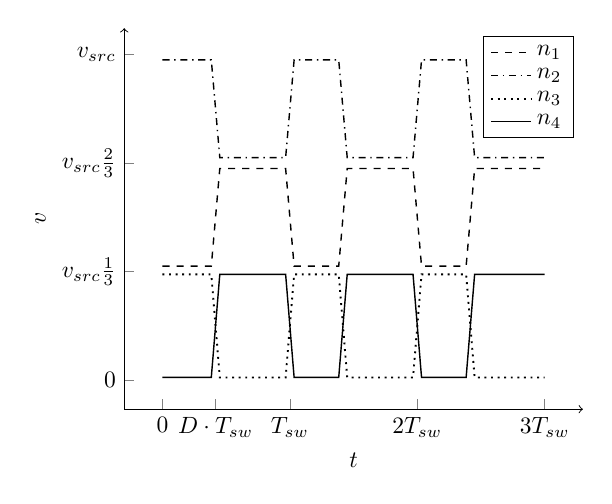
\begin{tikzpicture}[xscale=0.85, yscale=0.85]
    \begin{axis}[
        xlabel near ticks,
        xlabel=$t$,
        ylabel=$v$,
        axis line style={->},
        axis y line*=left,
        axis x line*=bottom,
        ytick = {0,2,4,6},
        yticklabels={0,$v_{src}\frac{1}{3}$,$v_{src}\frac{2}{3}$,$v_{src}$},
        xtick = {0,1.25,3,6,9},
        xticklabels={0,$D \cdot T_{sw}$,$T_{sw}$ ,$2 T_{sw}$,$3 T_{sw} $},
        ]

  %Vertical ticks
  %\draw (2pt,6) -- (-5pt,6) node[anchor=east]  {$v_{src} $};
  %\draw (2pt,4) -- (-5pt,4) node[anchor=east]  {$v_{src} \frac{2}{3}$};
  %\draw (2pt,2) -- (-5pt,2) node[anchor=east]  {$v_{src} \frac{1}{3}$};

  %Horizontal ticks
  %\draw (1.25,2pt) -- (1.25,-5pt) node[anchor=north]  {$DT$};
  %\draw (3,2pt) -- (3,-5pt) node[anchor=north]  {$T$};
  %\draw (6,2pt) -- (6,-5pt) node[anchor=north]  {$2T$};
  %\draw (9,2pt) -- (9,-5pt) node[anchor=north]  {$3T$};
  %\draw (0,0) node[anchor=north east]  {$0$};

  \addplot[semithick, dashed]
    plot coordinates{
        (0,2.1)   (1.15,2.1)  (1.35,3.9)  (2.9,3.9)
        (3.1,2.1) (4.15,2.1)  (4.35,3.9)  (5.9,3.9)
        (6.1,2.1) (7.15,2.1)  (7.35,3.9)  (9,3.9) };

  \addplot[semithick, dashdotted ]
    plot coordinates{
     (0,5.9)    (1.15,5.9)  (1.35,4.1)  (2.9,4.1)
     (3.1,5.9)  (4.15,5.9)  (4.35,4.1)  (5.9,4.1)
     (6.1,5.9)  (7.15,5.9)  (7.35,4.1)  (9,4.1)} ;

  \addplot[thick,dotted ]
    plot coordinates{
   (0,1.95)   (1.15,1.95)  (1.35,0.05)  (2.9,0.05)
   (3.1,1.95) (4.15,1.95)  (4.35,0.05)  (5.9,0.05)
   (6.1,1.95) (7.15,1.95)  (7.35,0.05)  (9,0.05)};

   \addplot[semithick]
    plot coordinates{
    (0,0.05)    (1.15,0.05)    (1.35,1.95)    (2.9,1.95)
    (3.1,0.05)  (4.15,0.05)  (4.35,1.95)  (5.9,1.95)
    (6.1,0.05)  (7.15,0.05)  (7.35,1.95)  (9,1.95) };

    \legend{$n_1$,$n_2$,$n_3$,$n_4$}


\end{axis}
\end{tikzpicture}
\caption{Transient voltage at the different \emph{pwm}-nodes of the 3:1 H-Dickson converter of Figure~\ref{fig:3_1_hscc}.}
\label{fig:pwm_nodes}
\end{SCfigure}

In fact, a H-SCC shares many of the characteristics of a buck converter, the most common LED driver circuit used in \emph{dc-dc} conversion. Adding the output filter to a SCC complements the converter providing tight current regulation, which overcomes the intrinsic limitation of SCC in current regulation. However it requires magnetic elements, challenging again the integrability  of the converter. The following sections introduces the characteristics of this new \emph{hybrid} topology as a LED driver, using the buck converter as a reference. %  since a H-SCC architecture can directly replace a buck converter LED driver providing the same regulation characteristics.

\begin{figure}[!h]
\centering
\ctikzset { bipoles/length=1cm}
%\ctikzset { scale=0.5}
\begin{subfigure}[t]{\textwidth}
    \centering
    %\ctikzset { bipoles/length=1cm}
        \begin{circuitikz}[american voltages,scale=0.6]
        \draw (-1,7) node[anchor=north]{ };
        \draw %Input Supply
                (-1,0)  to[V=$v_{src}$]
                %Draw Switches
                (-1,4)  --
                (4,4);

        %Capacitor C1
        \draw   (4,2) to[pC=$c_1$] (4,4);

        %Capacitor C2
        \draw (2,0)to[pC=$c_2$](2,2) --(4,2);

        %Capacitor C3
        \draw  (-1,0)--
               (6,0) to[pC=$c_3$]
               (6,2) -- (4,2);

         \draw (6,2) to[L,l=$l_o$,-o] (11,2) node[anchor=west] {};
         \draw (6,0) to[short,-o] (11,0) node[anchor=west] {};
         \draw (11,2) to[open,v^=$v_{out}$] (11,0);

         \draw (10,0) to[pC,l=$c_{o}$] (10,2);
         \draw (6,2) node[anchor=south] {$v_x$};

         \end{circuitikz}
     \subcaption{First phase, odd switches are closed and even switches are open.}
     \label{fig:hscc_full_p1}
     \end{subfigure}

\begin{subfigure}[t]{\textwidth}
      \centering
      \begin{circuitikz}[american voltages,scale=0.6]
        \draw (0,4.5) node[anchor=north]{ };
        \draw   %Input Supply
                (-1,0)  to[V=$v_{src}$]
                %Draw Switches
                (-1,4);

        \draw   (5,2) to[pC=$c_2$] (5,4);

        \draw %Capacitor C1
               (2,0)to[pC=$c_1$](2,4) --(5,4);

        \draw %Capacitor C3
               (5,0) to[pC=$c_3$]
               (5,2) -- (5,2);

         \draw (5,4) to[L,l=$l_o$,-o] (11,4) node[anchor=west] {};
         \draw (-1,0) to[short,-o] (11,0) node[anchor=west] {};
         \draw (11,4) to[open,v^=$v_{out}$] (11,0);
         \draw (10,0) to[pC,l=$c_{o}$] (10,4);

         \draw (5,4) node[anchor=south] {$v_x$};

         \end{circuitikz}
     \subcaption{Second phase, even switches are closed and odd switches are open.}
     \label{fig:hscc_full_p2}
     \end{subfigure}
\caption{The two switching modes of 3:1 H-Dickson of Figure~\ref{fig:3_1_hscc}}
\label{fig:hscc_phases}
\end{figure}

\subsection{Output Regulation}
\label{sec:out_reg}

In contrast with the classical SCC, the conversion ratio of a H-SCC converter depends on the duty cycle of the converter ($D$), consequently the conversion ratio can now be adjusted to provide regulation of the load without directly affecting the converter's efficiency.

Figure~\ref{fig:reg_comp} compares the idealized trend curves of the converter efficiency with respect to the conversion ratio for a H-SCC, a SCC and a buck converter. For example a 3:1 Dickson has an intrinsic conversion ratio of
$ m_i = \frac{1}{3} $ and provides regulation at costs of efficiency (see dashed line). Instead, using the third \emph{pwm}-node ($n_3$), located at the negative terminal of capacitor $c_1$ in the schematic of Figure~\ref{fig:3_1_hscc}, the converter has an adjustable conversion ratio of
\begin{equation}
m_3 = \frac{D}{3}
\end{equation}
by changing the duty cycle $D$ of the drive signal. In this case, the efficiency vs. regulation curve is flat within the regulation margins and drops for extreme duty cycles by cause of the internal losses of the SCC (see solid line). The details of the loss mechanisms in SCC and H-SCC are covered in chapter X dedicated to modeling. Indeed, the efficiency vs. regulation curve of a H-SCC is similar to the one of a buck converter (dotted line) but with a smaller dynamic range.
\begin{SCfigure}
\centering
\begin{circuitikz}[american voltages,xscale=0.55,yscale=0.65]
\begin{scope}
  \draw [->] (0,0) -- (10,0) node[anchor=north]{$m$};
  \draw [->] (0,0) -- (0,5.5) node[anchor=east]{$\eta$};

  %Vertical ticks
  \draw (2pt,4) -- (-5pt,4) node[anchor=east]  {$100\%$};
  \draw (2pt,2.5) -- (-5pt,2.5) node[anchor=east]  {$70\%$};

  %Horizontal ticks
  %\draw (1.25,2pt) -- (1.25,-5pt) node[anchor=north]  {$DT$};
  \draw (3,2pt) -- (3,-5pt) node[anchor=north]  {$\frac{1}{3}$};
  \draw (6,2pt) -- (6,-5pt) node[anchor=north]  {$\frac{2}{3}$};
  \draw (9,2pt) -- (9,-5pt) node[anchor=north]  {$1$};
  \draw (0,0) node[anchor=north east]  {$0$};

  \draw[thick, dashed] (0,0) --  (2.9,3.9) ;

  %\draw[thick, dotted] (0,0) --  (2.9,3.9) ;
  \draw[thick,dotted] (0.1,2) parabola[bend at end] (2,3.45) -- (6,3.7) parabola[bend at start] (8.9,1.5);

  \draw[thick] (0.1,1.75) parabola[bend at end] (0.75,3.5) -- (2.2,3.6) parabola[bend at start] (2.9,1.6);


  %\draw[thick, dashed] (0,3.375) -- (7.25,3.375) ;
  %\draw (2.075,3.375)node[anchor=north] {$\bar{v_x}$};

  %\draw[pil,<->] (8,4.1) -- (8,2.4) ;

  %\draw[dotted] (7.25,2.5) -- (8.1,2.5);

  %\draw (8,3.25) node[anchor=west] {$\Delta v_x$};
\end{scope}
\end{circuitikz}
\caption{Comparison of regulation vs. efficiency characteristics between converters: 3:1 H-Dickson $3rd$ \emph{pwm}-node (solid line), 3:1 Dickson (dashed line) and buck converter (dotted line).}
\label{fig:reg_comp}
\end{SCfigure}

\begin{table}[h]

\centering
\caption{Conversion ratio characteristics at the different nodes of a 3:1 H-Dickson converter}
\label{tab:3:1 H-Dick_M}
\renewcommand{\arraystretch}{1.5}% Wider
\begin{tabular}{l  c | c c c c c }
 Node &  & $n_1$ & $n_2$ & $n_3$ & $n_4$ & $n_{dc}$ \\
 \midrule
 Conversion ratio & $m_x$ & $\frac{2+D}{3} $    & $\frac{2-D}{3} $ & $\frac{D}{3} $ & $\frac{1-D}{3} $ & $\frac{1}{3}$ \\
 Range of conversion &       & $1 \cdots \frac{2}{3}$ & $\frac{2}{3} \cdots \frac{1}{3} $ & $\frac{1}{3} \cdots 0$ & $\frac{1}{3} \cdots 0 $ & - \\
 Dynamic conversion range & $\Delta m$ &  $\frac{1}{3}$ &  $\frac{1}{3}$ &  $\frac{1}{3}$ &  $\frac{1}{3}$ &  -
\end{tabular}
\end{table}

Ideally a buck converter provides a conversion ratio between 0 and 1. Indeed, it is the same case for a H-SCC, however the conversion ratio is segmented in different ranges. Each segment is associated with a different \emph{pwm}-node of the converter, and it has a limited dynamic range of regulation $\Delta m$. Table~\ref{tab:3:1 H-Dick_M} presents the conversion characteristics for the different nodes of the 3:1 H-Dickson of Figure~\ref{fig:3_1_hscc}. It can be seen that the dynamic range of conversion ($\Delta m$) is the same across all the \emph{pwm}-nodes and equal to the intrinsic conversion ratio of the converter $m_i$. This characteristic is shared between the two topologies used in this dissertation, Dickson and Ladder.

\subsection{Power Inductor}
\label{ch:power_inductor}

Like in a buck converter, a H-SCC uses a inductor-capacitor (LC) low pass filter to supply the a \emph{dc} voltage to the load. The use of an inductor challenges again the integrability of the converter, as it was already discussed in the second chapter, nevertheless the added advantages in terms of regulation and efficiency justify its use. At the same time, the inductor benefits from the reduced voltage ripple present in the \emph{pwm}-nodes, relaxing the requirements in terms of inductance and size.

The inductance value of the power inductor in a buck type converter configuration is
\begin{equation}
 l_{o}   = \frac{\Delta v_{x} \cdot DD'}{\Delta i f_{sw}},
\label{eq:gen_l}
\end{equation}
where $\Delta i$ is the \emph{peak-to-peak} current amplitude in the inductor, $D$ the duty cycle of the boost high side switch and $D'=(1-D)$. From eq.(\ref{eq:gen_l}) it can be seen that the size of the power inductor is directly proportional to the amplitude of the square-wave voltage at the switching node ($\Delta v_x$), which in a buck converter is equal to the source voltage as shown in the plot from Figure~\ref{fig:induc_vx}. Particularizing eq.(\ref{eq:gen_l}) for a buck converter, yields to
\begin{equation}
 l_{o,buck}  = \frac{v_{src} \cdot DD'}{\Delta i f_{sw} }.
\label{eq:buck_l}
\end{equation}

\begin{figure}[!h]
\centering
\ctikzset { bipoles/length=1cm}
\begin{subfigure}[t]{.45\textwidth}
    %\centering
    \raggedright
    \begin{circuitikz} [american voltages,scale=0.65]
    \draw
        (-1,0) to[V = $v_{src}$]
        (-1,4) -- (1,4) to[switch,l=$s_1$]
        (1,2) -- (1.5,2) to[inductor=${l_o}$,i=$i_o$]
        (3.5,2) -- (4,2) to[C,l=$c_o$] (4,0) -- (-1,0);

    \draw (4,2) to[short,-o] (5,2) node[anchor=west] {$v_o$};

    \draw (1,2) to[switch,l=$s_2$] (1,0);

    \draw (1,2) node[anchor=east] {$v_x$};

    \draw (0,-1) node[anchor=south] {};

    \end{circuitikz}
    \caption{}
    \label{fig:ind_ckt_l}
\end{subfigure}
\begin{subfigure}[t]{.45\textwidth}
    %\centering
    \raggedleft
    \begin{circuitikz} [scale=0.65]
    \begin{scope}%[xshift = 8cm, yshift=0cm]
        \draw[->] (0,0) -- (6.25,0) node[anchor=north] {$  t $};
        \draw[->] (0,0) -- (0,3.2) node[anchor= east] {$v_x $};

        %Ticks X
        \draw (2.75,2pt) -- (2.75,-5pt) node[anchor=north] {$T$};
        \draw (5.5,2pt) -- (5.5,-5pt) node[anchor=north] {$2T$};

        %Ticks Y
        \draw (2pt,2.5) -- (-5pt,2.5) node[anchor=east] {$v_{src}$};
        \draw (0,0) node[anchor=north east] {$0$};


        \draw[thick] (0,2.5) -- (1.25,2.5) -- (1.25,0) -- (2.75,0) -- (2.75,2.5) -- (4,2.5) -- (4,0) -- (5.5,0);
        \draw (0,-1) node[anchor=south] {};

        \draw[pil,<->] (4.75,-0.1) -- (4.75,2.6);
        \draw (4.75,1.25) node[anchor=west] {$\Delta v_x$};
        \draw[dotted] (4,2.5) -- (4.95,2.5);

    \end{scope}
    \end{circuitikz}
    \caption{}
\label{fig:induc_vx}
\end{subfigure}
\caption{Inductor based converter, \emph{left} - synchronous buck converter schematic; \emph{right} - transient voltage at the switching node during two switching periods. }
\label{fig:inductive_smps}
\end{figure}

Opposite to the buck converter, in the H-SCC the square-wave voltages are floating with respect the ground (see Figure~\ref{fig:vx_t}) and its ripple amplitude $\Delta v_x$ depends on the converter's topology. In the case of the Dickson and Ladder converters the amplitude of the voltage ripple $\Delta v_x$ is the same for all of the \emph{pwm}-nodes and equal to
\begin{equation}
 \Delta v_x   = m_i \cdot v_{src},
\label{eq:h_scc_Del_vx}
\end{equation}
therefore particularizing eq.(\ref{eq:gen_l}) for a Dickson or a Ladder H-SCC yields to
\begin{equation}
 l_{o,hscc}  = \frac{ m_i \cdot v_{src} \cdot DD'}{\Delta i f_{sw} }.
\label{eq:hscc_l}
\end{equation}
An important remark is that duty cycle in (\ref{eq:hscc_l}) and in (\ref{eq:buck_l}) are not correlated, therefore the two equations can not be directly compared.  Figure~\ref{fig:inductor_size} plots the normalized inductor values - $V_{src} = 1V$, $T_{sw}=1s$ and$\Delta i = 1A$- for Buck, 3:1 H-Dickson and 4:1 H-Dickson converters. The plot shows the symmetrical curve for the buck converter where the highest inductance value is when the converter operates at a half conversion ratio.
In contrast, the curves corresponding to the HSCCs present multiple parabolas, where each of them corresponds to a selected node of the HSCC converter. For instance, looking at the dashed line plotted for the 3:1 H-Dickson converter of Figure~\ref{fig:3_1_hscc}, the first parabola spans for a $m$ between $0$ and $1/3$ corresponds for an inductor connected to $n3$ or $n4$. The second parabola spans for a $m$ between $1/3$ and $2/3$ corresponds for an inductor is connected to $n2$. The last parabola spans for a $m$ between $2/3$ and $1$ corresponds when the inductor is connected to $n1$.
The reduction in inductance value with respect to the back converter spans out from half conversion ratio to the extremes where the inductance take the same values for all the converters.


\begin{SCfigure}
\centering
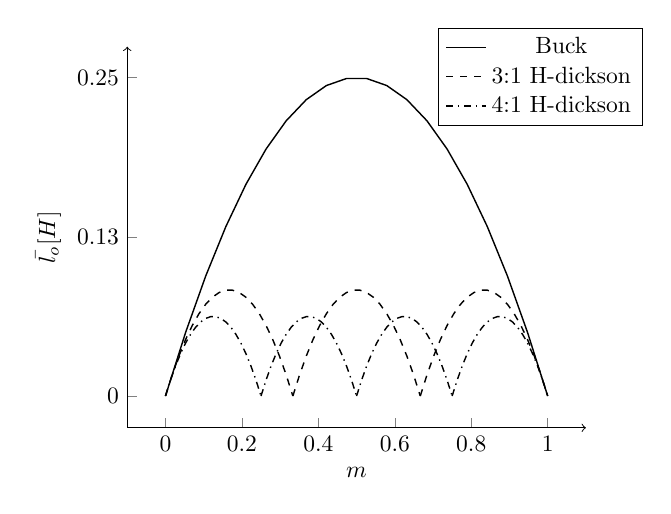
\begin{tikzpicture}[scale=0.85]
    \begin{axis}[
        xlabel near ticks,
        xlabel=$m$,
        ylabel={$\bar{l_o}  [ H ]  $} ,
        axis line style={->},
        axis y line*=left,
        axis x line*=bottom,
        ytick = {0,.125,.25},
        %yticklabels={0,$v_{src}\frac{1}{3}$,$v_{src}\frac{2}{3}$,$v_{src}$},
        domain=0:1,
        samples=20,
        %xticklabels={0,$D \cdot T_{sw}$,$T_{sw}$ ,$2 T_{sw}$,$3 T_{sw} $},
        legend style={at={(1.125,1.05)}, anchor= north east},
        ]

  \addplot [semithick] {x*(1-x)};
  \addplot [domain = 0:1/3,  semithick,dashed]   {1/3* (x*3)*(1-(x*3))};
  \addplot [domain = 0:1/4,    semithick,dashdotted]   {1/4* (x*4)*(1-(x*4))};

  \addplot [domain = 1/3:2/3,semithick,dashed] {1/3* (2-x*3)*(1-(2-x*3))};
  \addplot [domain = 2/3:1,  semithick,dashed]   {1/3* (x*3-2)*(1-(x*3-2))};


  \addplot [domain = 1/4:2/4,  semithick,dashdotted]   {1/4* (x*4 - 1)*(1-(x*4 - 1))};
  \addplot [domain = 2/4:3/4,  semithick,dashdotted]   {1/4* (3 - x*4)*(1-(3 - x*4))};
  \addplot [domain = 3/4:4/4,  semithick,dashdotted]   {1/4* (x*4-3)*(1-(x*4-3))};

  \legend {Buck, 3:1 H-dickson,4:1 H-dickson};
\end{axis}
\end{tikzpicture}
\caption{Inductance value for Buck, 3:1 H-Dickson and 4:1 H-Dickson converters as function of the conversion ratio; results are normalized  for $V_{src} = 1V$, $T_{sw}=1s$ and $\Delta i = 1A$.}
\label{fig:inductor_size}
\end{SCfigure}

The physical size of the inductor is proportional to the peak energy stored in it, and it can be computed from the maximum current through the inductor

\begin{equation}
 E_{l,max}  = \frac{1}{2} i_{max}^2 l_{o}.
\label{eq:eng_L}
\end{equation}

The minimum inductance value is when the converter operates in Boundary Conduction Mode (BCM) since the H-SCC is designed to operate in Continuous Conduction Mode (CCM). When a buck or H-SCC converter operates in BCM the minimum current is equal to zero and the peak current is equal to twice of the output current of the converter. Thus, the maximum inductor current is
\begin{equation}
 i_{max} = \Delta i  = 2 i_{out}
\label{eq:i_max}
\end{equation}

By substituting (\ref{eq:i_max}) and (\ref{eq:buck_l}) into (\ref{eq:eng_L}), the inductor peak energy for a buck can be found
\begin{equation}
E_{l,buck}  =   \frac{ i_{out} v_{src}  DD'}{f_{sw}}.
\label{eq:e_lmax_buck}
\end{equation}


\begin{SCfigure}
\centering
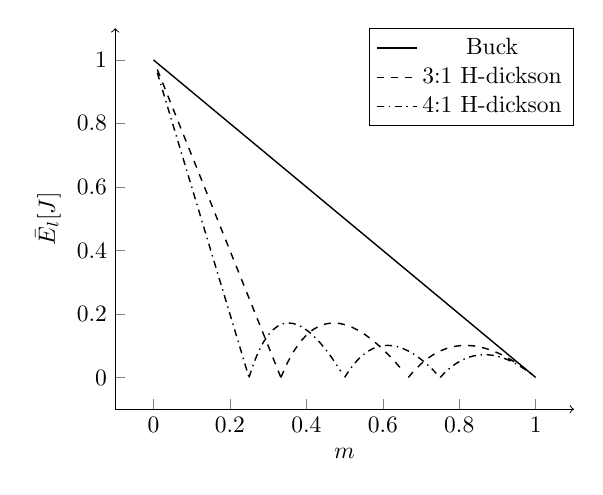
\begin{tikzpicture}[scale=0.85]
    \begin{axis}[
        xlabel near ticks,
        xlabel=$m$,
        ylabel={$\bar{E}_{l} [ J ]  $} ,
        axis line style={->},
        axis y line*=left,
        axis x line*=bottom,
        %ytick = {0,.125,.25},
        %yticklabels={0,$v_{src}\frac{1}{3}$,$v_{src}\frac{2}{3}$,$v_{src}$},
        domain=0:1,
        samples=20,
        %xticklabels={0,$D \cdot T_{sw}$,$T_{sw}$ ,$2 T_{sw}$,$3 T_{sw} $},
        legend style={at={(1,1)}, anchor= north east},
        ]

  \addplot [semithick] {(1-x)};

  \addplot [domain = 0.01:1/3,  semithick,dashed]   {1/x* 1/3* (x*3)*(1-(x*3))};
  \addplot [domain = 0.01:1/4,    semithick,dashdotted]   {1/x* 1/4* (x*4)*(1-(x*4))};

  \addplot [domain = 1/3:2/3-0.01,semithick,dashed] {1/x*1/3* (2-x*3)*(1-(2-x*3))};
  \addplot [domain = 2/3:1-0.01,  semithick,dashed]   {1/x*1/3* (x*3-2)*(1-(x*3-2))};


  \addplot [domain = 1/4:2/4-0.01,  semithick,dashdotted]   {1/x*1/4* (x*4 - 1)*(1-(x*4 - 1))};
  \addplot [domain = 2/4:3/4-0.01,  semithick,dashdotted]   {1/x*1/4* (3 - x*4)*(1-(3 - x*4))};
  \addplot [domain = 3/4:4/4-0.01,  semithick,dashdotted]   {1/x*1/4* (x*4-3)*(1-(x*4-3))};

  \legend {Buck, 3:1 H-dickson,4:1 H-dickson};
\end{axis}
\end{tikzpicture}
\caption{Peak energy storage for Buck, 3:1 H-Dickson and 4:1 H-Dickson converters as function of the conversion ratio;  results are normalized for $P_{out} = 1W$ and $f_{sw}=1Hz$.}
\label{fig:inductor_energy}
\end{SCfigure}


In a buck converter the source voltage can be written as
\begin{equation}
v_{src}  =  \frac{v_{out}} {D},
\label{eq:vo_buck}
\end{equation}
thus by substituting (\ref{eq:vo_buck}) into (\ref{eq:e_lmax_buck}), the $E_{l,buck}$ yields to
\begin{equation}
E_{l,buck}  =  \frac{v_{vout}}{D} \frac{ i_{out}  DD'}{f_{sw}} = \frac{(1-D)}{f_{sw}} P_{out}.
\label{eq:e_lmax_buck_II}
\end{equation}

By substituting (\ref{eq:i_max}) and (\ref{eq:hscc_l}) into (\ref{eq:eng_L}), the inductor peak energy for H-SCC with a Dickson or Ladder stages can be found
\begin{equation}
E_{l,hscc}  =   \frac{ m_{i} i_{out} v_{src}  DD'}{f_{sw}}.
\label{eq:e_lmax_hscc}
\end{equation}

In the hybrid Dickson and Ladder converters the source voltage is can be written as
\begin{equation}
v_{src}  =  \frac{v_{out}} {m},
\label{eq:vo_hscc}
\end{equation}
where $m$ is the conversion ratio of the converter. Thus by substituting (\ref{eq:vo_hscc}) into (\ref{eq:e_lmax_hscc}), the resutling expression of the inductor maximum energy yields to
\begin{equation}
E_{l,hscc}  =  \frac{v_{vout}}{m} \frac{ m_i i_{out}  DD'}{f_{sw}} = \frac{m_i D (1-D)}{m f_{sw}} P_{out}.
\label{eq:e_lmax_hscc_II}
\end{equation}



\begin{SCfigure}
\centering
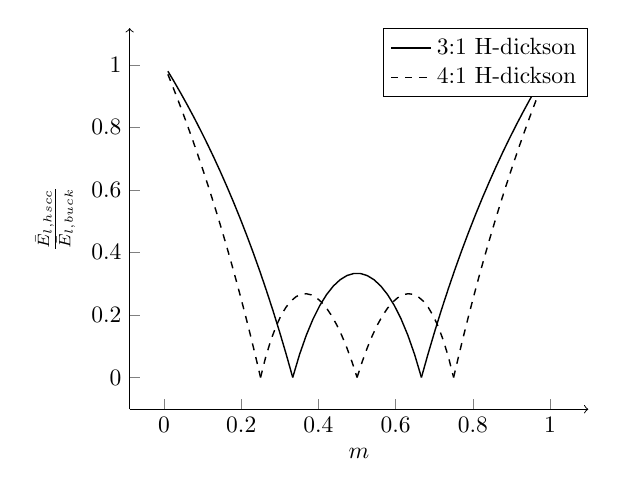
\begin{tikzpicture}[scale=0.85]
    \begin{axis}[
        xlabel near ticks,
        xlabel=$m$,
        ylabel={$ \frac{\bar{E}_{l,hscc}}{\bar{E}_{l,buck}}  $} ,
        axis line style={->},
        axis y line*=left,
        axis x line*=bottom,
        %ytick = {0,.125,.25},
        %yticklabels={0,$v_{src}\frac{1}{3}$,$v_{src}\frac{2}{3}$,$v_{src}$},
        domain=0:1,
        samples=20,
        %xticklabels={0,$D \cdot T_{sw}$,$T_{sw}$ ,$2 T_{sw}$,$3 T_{sw} $},
        legend style={at={(1,1)}, anchor= north east},
        ]


  \addplot [domain = 0.01:1/3,  semithick]   { (1/x* 1/3* (x*3)*(1-(x*3)))/(1-x) };
  \addplot [domain = 0.01:1/4,    semithick,dashed]   { (1/x* 1/4* (x*4)*(1-(x*4)))/(1-x)};

  \addplot [domain = 1/3:2/3,semithick] { (1/x*1/3* (2-x*3)*(1-(2-x*3)))/(1-x)};
  \addplot [domain = 2/3:1,  semithick]   { (1/x*1/3* (x*3-2)*(1-(x*3-2)))/(1-x)};


  \addplot [domain = 1/4:2/4,  semithick,dashed]   { (1/x*1/4* (x*4 - 1)*(1-(x*4 - 1)))/(1-x)};
  \addplot [domain = 2/4:3/4,  semithick,dashed]   { (1/x*1/4* (3 - x*4)*(1-(3 - x*4)))/(1-x)};
  \addplot [domain = 3/4:4/4,  semithick,dashed]   { (1/x*1/4* (x*4-3)*(1-(x*4-3)))/(1-x)};

  \legend {3:1 H-dickson,4:1 H-dickson};
\end{axis}
\end{tikzpicture}
\caption{Peak energy storage normalized with respect to a buck converter for a 3:1 H-Dickson and a 4:1 H-Dickson converters as function of the conversion ratio.}
\label{fig:inductor_normal}
\end{SCfigure}


Figure~\ref{fig:inductor_energy} plots (\ref{eq:e_lmax_buck_II}) and (\ref{eq:e_lmax_hscc_II}), both plots have the same trend of reducing the peak energy as the conversion ratio increases. As in the case of the inductance value (see Figure~\ref{fig:inductor_size}), the peak energy stored in the inductor is dramatically reduced, hence the volume, in case of using a H-SCC topology. In fact, normalizing the peak energy of the H-SCCs with respect to the buck, as shown in Figure~\ref{fig:inductor_normal}. The plot shows that the reduction in inductance spans from a conversion ratio of a half to the extremes symmetrically, being very effective in most of the conversion ratio range of the converter and decreasing at the two extremes. As the conversion ratio of the SCC increases the reduction in inductance increases and the effective region of reduction spans for a large range of conversion ratio.



\subsection{Power Switches}
The large number of switches used in a H-SCC has different advantages towards miniaturization of the converter. In fact, in a H-SCC the voltage stress applied to the different switches is a fraction of the input voltage, in contrast to the buck converter where each of the switches have to block the full input voltage. Therefore SCCs can be implemented with switches rated at lower voltages than the input voltage. Table ~\ref{tab:3:1 H-Dick_V_stress} shows the blocking voltages of the switches of the 3:1 H-Dickson of Figure~\ref{fig:3_1_hscc}.

\begin{table}[h]
\centering
\caption{Stress voltages at the switches of the 3:1 H-Dickson of Figure~\ref{fig:3_1_hscc}.}
\label{tab:3:1 H-Dick_V_stress}
\renewcommand{\arraystretch}{1.5}% Wider
\begin{tabular}{r  c }
 Switch \# & Stress voltage  \\
 \midrule
 $s_1,s_3 \cdots s_7$ & $\frac{1}{3} v_{src}$ \\
 $s_2$ & $\frac{2 }{3} v_{src}$
\end{tabular}
\end{table}

Reducing the voltage stress has several advantages. First, low voltage devices take less silicon area in the standard integration processes. Second, switching performance of these devices is better since they are smaller in area, and with less parasitic capacitances, as a consequence, they can switch faster. Finally, the switching losses of the converter are reduced since they keep a quadratic proportion with blocking voltages of the switches ($v_{ds}$). The reduction of the switching loss with respect to a buck converter can be easily calculated using the switching loss formula associated to parasitic  capacitances~\cite{2001Erickson}:
\begin{equation}
P_{sw} = \frac{1}{2} f_{sw} \cdot c_{ds} \cdot v_{ds}^2.
\label{eq:p_sw_dev}
\end{equation}
In this exercise it has been assumed that $c_{ds}$ is equal for the different switches in both converters, despite the fact that value would be different for each switch in a real implementation. This simplification has been taken in order to show the impact of the voltage reduction to the switching loss. %Actually, as previously mentioned using lower voltage switches will also lead in a reduction to the parasitic capacitances leading to smaller switching loss as well.

The blocking voltage of the switch in the buck converter of Figure~\ref{fig:ind_ckt_l} is $v_{src}$, thus replacing it in (\ref{eq:p_sw_dev}), the switching losses are
\begin{equation}
P_{sw,buck} =   f_{sw} \cdot c_{ds} \cdot v_{src}^2.
\label{eq:p_sw_buck}
\end{equation}

The blocking voltages of the 3:1 H-Dickson are in table~\ref{tab:3:1 H-Dick_V_stress}, thus replacing it in (\ref{eq:p_sw_dev}) the switching losses for that converter are
\begin{equation}
P_{sw,hscc} =  \frac{6}{2}  f_{sw} \cdot c_{ds} \left( \frac{1}{3} v_{src} \right)^2 + \frac{1}{2}  f_{sw} \cdot c_{ds} \left( \frac{2}{3} v_{src} \right)^2 ,
\label{eq:p_sw_hscc}
\end{equation}
rearranging yields to
\begin{equation}
P_{sw,hscc} =  \frac{5}{9}  f_{sw} \cdot c_{ds} \cdot v_{src}^2.
\label{eq:p_sw_hscc_sol}
\end{equation}

Dividing (\ref{eq:p_sw_buck}) and (\ref{eq:p_sw_hscc_sol}) yields the switching loss ratio between the two converters:
\begin{equation}
\frac{P_{sw,hscc}}{P_{sw,buck}} =  \frac{5}{9}  f_{sw} \cdot c_{ds} \cdot v_{src}^2.
\label{eq:p_sw_hscc_sol}
\end{equation}

The results for a generalized $N$:1 Dickson and Ladder converter are in table~\ref{tab:Dick_Ladder_v_blk}, and in Figure~\ref{fig:psw_ratio} is plotted the switching loss ratio with respect to the buck converter.
\begin{table}[h]
\centering
\caption{Switch blocking voltage of Dickson and Ladder converters.}
\label{tab:Dick_Ladder_v_blk}
\renewcommand{\arraystretch}{1.5}% Wider
\begin{tabular}{r | c  c   }
 Converter &  N:1 Dickson  $ N \geq$ 3  &  N:1 Ladder $ N \geq 2$  \\
 \midrule
\# Switches & $ 4 + N $  & $2 \cdot N$ \\
 $v_{ds}$ & $\begin{array} {rcl} \frac{v_{src}}{N}   & \to &  6~ \text{switches} \\
                                           \frac{2 v_{src}}{N} & \to &  (N - 2) ~\text{switches}
                       \end{array}$
                       &   $ \frac{v_{src}}{N} $ \\
 $ P_{sw}$ &  $ \frac{4+N}{8 \cdot N^2} \cdot v_{vin}^2 \cdot f_{sw}  \cdot {c_{ds}} $ &  $ \frac{1}{ N} \cdot v_{src}^2 \cdot f_{sw} \cdot {c_{ds}} $  \\
 $ \frac{P_{sw}}{P_{sw,buck}}$ &  $ \frac{4+N}{8 \cdot N^2}  $ &  $ \frac{1}{ N}  $  \\


 \end{tabular}
\end{table}

Both converters achieve a reduction of the switching losses with respect to the buck converter. In fact the switching loss decrease as $N$ increases, although the number of switches increase as well. Reducing the switching loss enables to operate the converter at higher frequencies, thus with a smaller switching period $T_{sw}$, which is also effective in the reduction of the power inductor.

\begin{SCfigure}
\centering
\begin{tikzpicture}[scale=0.7]
    \begin{axis}[
        xlabel near ticks,
        xlabel=$N$,
        ylabel=$P_{sw}/P_{sw,buck}$,
        axis line style={->},
        axis y line*=left,
        axis x line*=bottom,
        %ytick = {0,2,4,6},
        %yticklabels={0,$v_{src}\frac{1}{3}$,$v_{src}\frac{2}{3}$,$v_{src}$},
        domain=3:10,
        samples=7,
        %xticklabels={0,$D \cdot T_{sw}$,$T_{sw}$ ,$2 T_{sw}$,$3 T_{sw} $},
        ]

  %\addplot [semithick] {x*0+1};
  \addplot [semithick,mark=o,mark size=2,scale plot marks=false] {(4+x)/(8*x^2)};
  \addplot [semithick,mark=square, mark size=2 ,scale plot marks=false]{1/x};
  \legend {Dickson,Ladder};
\end{axis}
\end{tikzpicture}
\caption{Switching loss ratio for Dickson and Ladder converters with respect to buck converter.}
\label{fig:psw_ratio}
\end{SCfigure}

There are a couple of considerations regarding these results for a practical implementation of a H-SCC. On the one hand, they are obtained assuming that $c_{ds}$ is the same for all the switches in both converters. In a practical converter each device has a different $c_{ds}$ value defined by two of the device parameters; $c_{ds}$ is directly proportional to the rated $v_{ds}$  voltage and inversely proportional to the channel resistance $r_{on}$. Theoretically lower voltage switches have smaller $c_{ds}$, but the final value will also depends on its $r_{on}$. On the other hand, H-SCC has a larger number of devices in series in the current path compared to a buck that only has only one switch in the current path in both phases. A proper H-SCC design reduces the number of switches in the high current path, helping to keep the conduction loss low. %Further considerations about this are explained in  section~\ref{sc:high_current_path}.



\subsection{Multiple Outputs}

The use of the internal nodes of the SCC allows to provide multiple outputs with a single power train. In this case the converter could be simultaneously loaded at the \emph{pwm}-nodes and at the \emph{dc}-node, providing different conversion ratio for each output. The conversion ratio at the \emph{dc}-node (or nodes)  is given by the intrinsic conversion ratio of the converter $m_i$, independent of the variations in the duty cycle of the driving signal, yet the fixed output can be linear regulated to adjust the output voltage.  The conversion ratio for the other \emph{pwm}-nodes is function of $D$ and determined in each node by the node conversion ration $m_n$. In the case of using multiple \emph{pmw}-nodes, all the outputs will depend on $D$, hence it will not be possible to have independent regulation for each of the outputs.

\begin{figure}[!h]
\centering
\ctikzset { bipoles/length=1cm}
\begin{circuitikz}[american voltages,scale=0.65]
\draw
        %Draw Switches

        (0,0) node[sground]{} to[V=$v_{src}$]
        (0,8)  --
        (5,8)   to[switch,l_=$s_1$,-*]
        (5,6)   to[switch,l_=$s_2$]
        (5,4)   to[switch,l_=$s_3$]
        (5,2)   to[switch,l_=$s_4$]
        (5,0)  --
        (0,0)

        (5,6) to[short] (8,6) to[L,l=$l_o$] (12,6) to[C,l_=$c_o$] (12,3) node[sground]{}
        (11,6) -- (14,6) to[R,l_=$r_2$,v^=$v_{o2}$] (14,3) node[sground]{}

        (5,4) to[short]
        (9,4) to[R,l_=$r_1$,v^=$v_{o1}$] (9,0) -- (5,0)

%Draw Capacitors
        (5,2) --
        (3,2) to[C=$c_{fly}$]
        (3,6)--
        (5,6)

        (5,0) --
        (7,0) to[C,l=$c_{dc}$]
        (7,4)--
        (5,4);

\end{circuitikz}
\caption {2:1 H-SCC with two outputs; $r_1$ is supplied by the \emph{dc}-node and $r_2$ is supplied by the first \emph{pwm}-node.}
\label{fig:2:1hscc_dual_output}
\end{figure}

Figure~\ref{fig:2:1hscc_dual_output} shows a converter with two output voltages. $r_1$ is connected to the \emph{dc}-node with an output voltage approximated to
\begin{equation}
v_{o1} = \frac{1}{2} v_{src}.
\end{equation}

$r_2$ is connected to the first \emph{pwm}-node with an output voltage function of $D$ as
\begin{equation}
v_{o2} = \frac{1+D}{2} v_{src},
\end{equation}
thus this output can be regulated.

%\subsection{Topology configurations}
%
%Here will be studied the different possibilities that this topology offers. It has to be considered the different combinations N:1 SCC  [Buck, Boost, Buck-Boost], 1:N SCC [Buck,Boost, Buck-Boost].


\section{LED Driver}

The buck is one of the most used converter as LED driver in \emph{dc-dc} applications. The buck converter has an excellent current regulation and a continuous output current thanks to the inductor connected in series with the LEDs as shown in Figure~\ref{fig:ind_ckt_led_drv}.

\begin{figure}[!h]
\centering
\ctikzset { bipoles/length=1cm}
\begin{subfigure}[t]{.45\textwidth}
    %\centering
    \raggedright
    \begin{circuitikz} [american voltages,scale=0.65]
    \draw
        (-1,0) to[V = $v_{src}$]
        (-1,4) -- (1,4) to[switch,l_=$s_1$]
        (1,2) -- (1.5,2) to[inductor=${l_o}$,i=$i_o$]
        (3.5,2) -- (4,2) to[C,l_=$c_o$] (4,0) -- (-1,0);

    \draw (4,2) to[short] (5.5,2) to[leD*,v_=$v_o$] (5.5,0) -- (4,0);

    \draw (1,2) to[switch,l_=$s_2$] (1,0);

    \draw (1,2) node[anchor=east] {$v_x$};

    \draw (0,-1) node[anchor=south] {};

    \end{circuitikz}
    \caption{}
    \label{fig:ind_ckt_led_drv}
\end{subfigure}
\hfill
\begin{subfigure}[t]{.45\textwidth}
    %\centering
    \raggedleft
    \begin{circuitikz} [scale=0.65]
    \begin{scope}%[xshift = 8cm, yshift=0cm]
        \draw[->] (0,0) -- (6.25,0) node[anchor=north] {$  t $};
        \draw[->] (0,0) -- (0,3.2) node[anchor= east] {$v_x $};

        %Ticks X
        \draw (2.75,2pt) -- (2.75,-5pt) node[anchor=north] {$T$};
        \draw (5.5,2pt) -- (5.5,-5pt) node[anchor=north] {$2T$};

        %Ticks Y
        \draw (2pt,2.5) -- (-5pt,2.5) node[anchor=east] {$v_{src}$};
        \draw (0,0) node[anchor=north east] {$0$};


        \draw[thick] (0,2.5) -- (1.25,2.5) -- (1.25,0) -- (2.75,0) -- (2.75,2.5) -- (4,2.5) -- (4,0) -- (5.5,0);
        \draw (0,-1) node[anchor=south] {};

        \draw[pil,>-<] (4.78,1.65) -- (4.78,0.6);
        \draw (4.78,0.55) -- (4.78,1.85)node[anchor=west] {$\Delta v_f$};



        \draw[thick,dotted] (0,1.36) -- (6,1.36) ;
        \draw[thick,dotted] (0,0.9) -- (6,0.9) ;
        \draw[thick,dashed] (0,1.137) -- (6,1.137) node[anchor=west] {$\bar{v_o}$};

    \end{scope}
    \end{circuitikz}
    \caption{}
\label{fig:induc_vx_led_drv}
\end{subfigure}
\caption{\emph{Left} - buck based LED driver schematic; \emph{right} - transient voltage at the switching node(thick line), average output voltage (dashed line), and forward voltage limits (dotted lines). }
\label{fig:inductive_led_drv}
\end{figure}

It can be seen in Figure~\ref{fig:induc_vx_led_drv} that the voltage swing at the switching node ($v_x$) of a buck converter goes from ground to $v_{src}$ providing the full conversion ratio range, between 0 and 1. Actually, this regulation range is often wider than the margins of variation in the LED's forward voltage (marked by the discontinuous lines in Figure~\ref{fig:induc_vx_led_drv}), as previously discussed in section~\ref{sc:LED_load}.

\begin{figure}[!h]
\centering
\ctikzset { bipoles/length=1cm}
\begin{subfigure}[t]{.45\textwidth}
    %\centering
    \raggedright
    \begin{circuitikz} [american voltages,scale=0.65]
    \draw[dotted] (1,4) -- (1,3.5);

    \draw (1,3.35) -- (0.5,3.35);
    \draw[dotted] (0.5,3.35) --  (-.25,3.35) -- (-.25,3);

    \draw
        (1,3.5) to[switch,l_=$s_2$]
        (1,2) -- (2,2) to[inductor=${l_o}$,i=$i_o$]
        (4,2) -- (4,2) to[C,l_=$c_o$] (4,0.5) node[sground]{};

    \draw (4,2) to[short] (5.5,2) to[leD*,v_=$v_o$] (5.5,0.5) node[sground]{};

    \draw (1,2) to[switch,l_=$s_3$] (1,0.5);
    \draw[dotted] (1,0.5) --  (1,0) ;

    \draw (1.75,2) -- (1.75,1.5);
    \draw[dotted] (1.75,1.5) -- (1.75,1);

    \draw (1,2) node[anchor=east] {$v_x$};

    \draw (0,-1) node[anchor=south] {};

    \end{circuitikz}
    \caption{}
    \label{fig:hscc_ckt_led_drv}
\end{subfigure}
\hfill
\begin{subfigure}[t]{.45\textwidth}
    %\centering
    \raggedleft
    \begin{circuitikz} [scale=0.65]
    \begin{scope}%[xshift = 8cm, yshift=0cm]
        \draw[->] (0,0) -- (6.25,0) node[anchor=north] {$  t $};
        \draw[->] (0,0) -- (0,3.2) node[anchor= east] {$v_x $};

        %Ticks X
        \draw (2.75,2pt) -- (2.75,-5pt) node[anchor=north] {$T$};
        \draw (5.5,2pt) -- (5.5,-5pt) node[anchor=north] {$2T$};

        %Ticks Y
        \draw (2pt,2.5) -- (-5pt,2.5) node[anchor=east] {$v_{src}$};
        \draw (2pt,1.67) -- (-5pt,1.67) node[anchor=east] {$v_{src} \frac{2}{3}$};
        \draw (2pt,0.83) -- (-5pt,0.83) node[anchor=east] {$v_{src} \frac{1}{3}$};
        \draw (0,0) node[anchor=north east] {$0$};


        \draw[thick] (0,1.67) -- (1.25,1.67) -- (1.25,0.83) -- (2.75,0.83) -- (2.75,1.67) -- (4,1.67) -- (4,0.83) -- (5.5,0.83);
        \draw (0,-1) node[anchor=south] {};

        \draw[pil,>-<] (4.78,1.65) -- (4.78,0.6);
        \draw (4.78,0.55) -- (4.78,1.85)node[anchor=west] {$\Delta v_f$};



        \draw[thick,dotted] (0,1.36) -- (6,1.36) ;
        \draw[thick,dotted] (0,0.9) -- (6,0.9) ;
        \draw[thick,dashed] (0,1.137) -- (6,1.137) node[anchor=west] {$\bar{v_o}$};

    \end{scope}
    \end{circuitikz}
    \caption{}
\label{fig:hscc_vx_led_drv}
\end{subfigure}
\caption{\emph{Left} - switching node detail of a 3:1 H-Dickson based LED driver; \emph{right} - transient voltage at the switching node(thick line), average output voltage (dashed line), and forward voltage limits (dotted lines).  }
\label{fig:hscc_led_drv}
\end{figure}

The abrupt $v-i$ characteristics of the LEDs is an advantage for the reduced conversion range of the H-SCC. Opposite to the buck converter, the H-SSCC has a narrower voltage swing at the switching node. Figure~\ref{fig:hscc_led_drv} shows in a H-SCC  the voltage swing can be reduced just to provide the necessary regulation margins for the LED. As described in the previous section~\ref{sec:out_reg}, the dynamic conversion range at the outputs depend on the intrinsic conversion ratio ($m_i$) of the SCC stage, therefore it can be adjusted for the requirements of the load. Additionally, reducing the dynamic conversion range reduced the voltage swing at the inductor, which at the same time, relaxes the requirements of the output inductor (see section~\ref{ch:power_inductor}).

The following subsections present different LED drivers based on H-SCCs for \emph{dc-dc} and \emph{ac-dc}. Actually, they are also suitable to supply any other type of load, specially when it requires reduced regulation margins, but it will not be covered in this dissertation.

\subsection{Single-stage \emph{dc-dc} with auxiliary output voltage}

Figure~\ref{fig:5_1_hscc_emerge} shows the \emph{dc-dc} LED driver with an auxiliary output voltage~\cite{WO2015/040564}.
In fact, this architecture has been used in an experimental set-up for this dissertation presented in the last chapter. The converter features two outputs: The main output $v_{out}$ supplies the LED load and normally delivers the largest amount of power of the converter. The output voltage can be controlled using the duty cycle $D$, thus its value is given by
\begin{equation}
v_{out} =  v_{src}  \frac{4 - D }{5}.
\label{eq:dc_dc_vout}
\end{equation}

The secondary output $v_{aux}$ supplies the low voltage electronics dedicated for the control of the driver, providing functionalities such as connectivity, light control or stand by operation. The secondary output has not direct means of regulation and provides a fix conversion ratio equal to
\begin{equation}
v_{aux} =  v_{src} \frac{1 }{5}.
\label{eq:dc_dc_vaux}
\end{equation}

\begin{figure}[t]
\ctikzset { bipoles/length=1cm}

\centering
    \begin{circuitikz}[american voltages,scale=0.6]

    \draw
            %Input Supply
            (-1,0)  to[V=$v_{src}$]
            %Draw Switches
            (-1,14)  --
            (5,14)  to[switch=$s_1$] %node[anchor=west] {$n_1$}%S1
            (5,12)  to[switch=$s_2$] %node[anchor=east] {$n_2$}%S1
            (5,10)  to[switch=$s_3$] %node[anchor=east] {$n_3$}%S1
            (5,8)   to[switch=$s_4$] %node[anchor=west] {$n_4$}%S2
            (5,6)   to[switch=$s_5$] %node[anchor=west] {$n_5$}%S3
            (5,4) --
            %left branch
            (3,4)   to[switch=$s_9$]
            (3,2)   to[switch=$s_8$]
            (3,0);

    \draw   %right branch
            (5,4) --
            (7,4)   to[switch,l_=$s_6$]
            (7,2)   to[switch,l_=$s_7$]
            (7,0) -- (-1,0);



    \draw %Capacitor C1
           (2,8)
            to[pC,l_=$c_1$] (2,12) --
           (5,12);

    \draw %Capacitor C2
           (8.25,6)  to[pC,l_=$c_2$](8.25,10) --
           (5,10);

    \draw %Capacitor C3
           (3,2) -- (2,2)
            to[pC,l_=$c_3$] (2,8) --
           (5,8);

    \draw %Capacitor C4
           (7,2) --
           (8.25,2) -- (8.25,4) to[pC,l_=$c_4$](8.25,6) --
           (5,6);


    \draw  %LC output filter &  Output LED string
            (8.25,10)node[anchor=south] {$v_x$} to[L=$l_o$] (14,10)
            (13.5,0) to[pC,l=$c_{o}$] (13.5,10) -|
            (16,9) to[leD*] (16,7) to[leD*] (16,5) to[leD*] (16,3) to[leD*] (16,1) |- (7,0) ;

    %Vout label
    \draw (16.25,12) to[open,v^=$v_{out}$] (16.25,-2);

    \draw %Capacitor C3
           (5,0) to[pC,l_=$c_5$,-*] (5,4) ;% node[anchor=south east] {$n_{dc}$};

     %\draw (7,4) to[short,-o] (10,4) node[anchor=west] {};
     %\draw (7,0) to[short,-o] (12,0) node[anchor=west] {};


     \draw (7,4) --([hs]8.25,4 |- 7,4) arc(180:0:\radius) to[short,-o] (10,4) to[open,v^=$v_{aux}$] (10,0) ;


     \end{circuitikz}
 \caption{ 5:1 Dickson LED driver for 24V e-merge track lighting application. The driver has two outputs: A $12V$, $12W$  LED string, and a $4V$, $200mW$  to supply low voltage loads. }
 \label{fig:5_1_hscc_emerge}
\end{figure}
Nevertheless, the voltage at this output can be still controlled by means of a linear regulator.

This architecture has a limited conversion range, between $3/5$ and $4/5$. The conversion ratio can be extended introducing a multiplexer between the different floating \emph{pwm}-nodes and the power inductor~\cite{WO2015/040517} as shown in Figure~\ref{fig:5_1_hscc_mux}. The multiplexer allows to connect any of available \emph{pwm}-nodes of the converter with the power inductor, in that way the conversion ratio of the converter covers the entire dynamic range of conversion between ground and $v_{src}$. A detailed description of this architecture can be found in the annex X section Y.

\begin{figure}[t]
\ctikzset { bipoles/length=1cm}

\centering
    \begin{circuitikz}[american voltages,scale=0.6]

    \draw
            %Input Supply
            (0,0)  to[V=$v_{src}$]
            %Draw Switches
            (0,14)  --
            (5,14)  to[switch=$s_1$] %node[anchor=west] {$n_1$}%S1
            (5,12)  to[switch=$s_2$] %node[anchor=east] {$n_2$}%S1
            (5,10)  to[switch=$s_3$] %node[anchor=east] {$n_3$}%S1
            (5,8)   to[switch=$s_4$] %node[anchor=west] {$n_4$}%S2
            (5,6)   to[switch=$s_5$] %node[anchor=west] {$n_5$}%S3
            (5,4) --
            %left branch
            (3,4)   to[switch=$s_9$]
            (3,2)   to[switch=$s_8$]
            (3,0);

    \draw   %right branch
            (5,4) --
            (7,4)   to[switch,l_=$s_6$]
            (7,2)   to[switch,l_=$s_7$]
            (7,0) -- (0,0);



    \draw %Capacitor C1
           (2,8)
            to[pC,l_=$c_1$] (2,12) --
           (5,12);

    \draw %Capacitor C2
           (8.25,6)  to[pC,l=$c_2$](8.25,10) --
           (5,10);

    \draw %Capacitor C3
           (3,2) -- (2,2)
            to[pC,l_=$c_3$] (2,8) --
           (5,8);

    \draw %Capacitor C4
           (7,2) --
           (8.25,2) -- (8.25,4) to[pC,l=$c_4$](8.25,6) --
           (5,6);


    \draw  %LC output filter &  Output LED string
            (12,10)node[anchor=south west] {$v_x$} to[L=$l_o$] (15.5,10)
            (15.5,0) to[pC,l=$c_{o}$] (15.5,10) -|
            (18,9) to[leD*] (18,7) to[leD*] (18,5) to[leD*] (18,3) to[leD*] (18,1) |- (7,0) ;

            %Mux
    \draw   (12,10) -- (12,11) -- (11,11.5) -- (11,8.5) -- (12,9) -- (12,10)
            (11.5,10) node[rotate=90] {$mux$}
            (11.5,11.25) -- (11.5,12) node[anchor=west, rotate=90] {$sel$};

    \draw    %Mux connections
            (5,12)  --  (10,12) |- (11,11)
            (8.25,10)  --  (11,10)
            (5,8) --  (6.5,8) -- ([vs_d]5,10 -| 6.5,8 ) arc(270:90:\radius) --  (6.5,10.5) -- (11,10.5)
            (8.25,6) -| (9.5,9.5) -- (11,9.5)
            (8.25,2) -| (10,9) -- (11,9);

    %Vout label
    \draw (16.25,12) to[open,v^=$v_{out}$] (16.25,-2);

    \draw %Capacitor C3
           (5,0) to[pC,l_=$c_5$] (5,4) ;% node[anchor=south east] {$n_{dc}$};

     %\draw (7,4) to[short,-o] (10,4) node[anchor=west] {};
     %\draw (7,0) to[short,-o] (12,0) node[anchor=west] {};


     %\draw (7,4) --([hs]8.25,4 |- 7,4) arc(180:0:\radius) to[short,-o] (10,4) to[open,v^=$v_{aux}$] (10,0) ;
     \end{circuitikz}
 \caption{ 5:1 H-Dickson LED driver with a multiplexer that enables to connect the different switching nodes with the power inductor.  }
 \label{fig:5_1_hscc_mux}
\end{figure}

\subsection{Single-stage \emph{ac-dc}}

The H-SCC can be also used in different \emph{ac-dc} applications with few modifications of the original architecture. In \emph{ac-dc} conversion the power converter must be able to converter a substantial range of the mains voltage to keep high power factor (PF) and low total harmonic distortion (THD). On of the most common practices is to use a boost converter to step-up the input voltage above the mains peak voltage, in that way the input voltage is always below the output voltage allowing the converter to operate for the entire range of the input voltage.

A H-SCC converter can also operate as a boost converter just by swapping the input and the output ports, and by adding a multiplexer, the converter can cover the full range of conversion between 1 to $\infty$ like a boost converter. Figure~\ref{fig:hscc_boost} shows a boost 1:3 H-Dickson converter with a multiplexer.

Table~\ref{tab:1:3 H-Dick_M} presents the conversion ratios associated to each of the nodes. Notice that the conversion ratio for the \emph{dc}-node ($n_{dc}$) is not a gain, in reality it is smaller than one, $1/3$ in this case, the same as for the 3:1 H-Dickson. The reason for that is because the voltage at the output ($v_{out}$) fixes the voltage value at capacitors and \emph{pwm}-nodes, hence the conversion ratio for \emph{dc}-node is taken with respect to the output voltage $v_{out}$ and not form the input $v_{src}$.

\begin{figure}[t]
\ctikzset { bipoles/length=1cm}
\centering
    \begin{circuitikz}[american voltages,scale=0.6]

    \draw
            %Input Supply
            (-4,0)--
            (11,0)  to[pC,l=$c_{o}$]
            %Draw Switches
            (11,10)  --
            (5,10)  to[switch=$s_1$] %S1
            (5,8)   to[switch=$s_2$] %S2
            (5,6)   to[switch=$s_3$] %S3
            (5,4) --
            %left branch
            (3,4)   to[switch=$s_7$]
            (3,2)   to[switch=$s_6$]
            (3,0);

    \draw   (11,10) -| (13,9) to[leD*] (13,7) to[leD*] (13,5) to[leD*] (13,3) to[leD*] (13,1) |- (7,0) ;
    \draw    (13.25,12) to[open,v^=$v_{out}$] (13.25,-2);

    \draw   %right branch
            (5,4) --
            (7,4)   to[switch,l_=$s_4$]
            (7,2)   to[switch,l_=$s_5$]
            (7,0);

    % Nodes
    \draw   (5,8) node[anchor=west] {$n_1$};
    \draw   (8.25,6) node[anchor=south] {$n_2$};
    \draw   (2,2) node[anchor=north] {$n_3$};
    \draw   (8.25,2) node[anchor=west] {$n_4$};



    \draw %Capacitor C1
           (3,2) -- (2,2)
            to[pC,l_=$c_1$] (2,8) --
           (5,8);

    \draw %Capacitor C2
           (7,2) --
           (8.25,2)  to[pC,l_=$c_2$](8.25,6) --
           (5,6);

    %\draw  %Inductor
    %        (8.25,6) to[L=$l_o$,-o] (12,6);


    \draw %Capacitor C3
           (5,0) to[pC,l_=$c_3$] (5,4) node[anchor=south east] {$n_{dc}$};

     %\draw (7,4) to[short,-o] (10,4) node[anchor=west] {};
     %Inductor
     \draw (-4,0) to[rsV=$v_{src}$]
           (-4,6) to[L=$l_i$] node[anchor=south] {$v_x$} (-1,6);

     %Mux connections
     \draw (2,8) -|  (1,7) -- (0.25,7) node[anchor=east] {$_3$}%top 1
           (0.25,6) node[anchor=east] {$_2$} -- ([hs]1,6 -| 2,2 ) arc(180:0:\radius) -- (5,6)%middle
           (2,2) -| (1,5) -- (0.25,5) node[anchor=east] {${_1}$}; % bottom 1
     %mux
     \draw (-1,5) -- (-1,7) -- (0.25,7.5) -- (0.25,4.5) -- (-1,5)
           (-0.6,6) node[rotate=90] {mux}
           (-0.6,7.2) -- (-0.6,8) node[anchor=west,rotate=90] {sel};



     \end{circuitikz}
 \caption{ H-SCC boost  with a 1:3 H-Dickson topology with a multiplexer.}
 \label{fig:hscc_boost}
\end{figure}

\begin{table}[h]
\centering
\caption{Conversion ratio characteristics at the different nodes of a 1:3 H-Dickson converter.}
\label{tab:1:3 H-Dick_M}
\renewcommand{\arraystretch}{1.5}% Wider
\begin{tabular}{l  c | c c c c c }
 Node &  & $n_1$ & $n_2$ & $n_3$ & $n_4$ & $n_{dc}$\footnote{Conversion ratio for the \emph{dc}-node is taken with respect to $v_{out}$} \\
 \midrule
 Conversion ratio & $m_x$ & $\frac{3}{2+D} $    & $\frac{3}{2-D} $ & $\frac{3}{D} $ & $\frac{3}{1-D} $ & $\frac{1}{3}$ \\
 Range of conversion &       & $1 \cdots \frac{3}{2}$ & $\frac{3}{2} \cdots 3 $ & $3 \cdots \infty $ & $ 3 \cdots \infty $ & - \\
 Dynamic conversion range & $\Delta m$ &  $\frac{1}{2}$ &  $\frac{3}{2}$ &  $\infty$ &  $\infty$ &  -
\end{tabular}
\end{table}

This architecture converts rectified mains voltage to a \emph{dc} voltage and enables current regulation at the load. The  circuit operates by sections, in this case 3, in order to cover the full range of the input voltage.  Depending on the input voltage and the bus voltage the multiplexer switch channel accordingly. When the input voltage ($v_{src}$) is between $0$  and $ \frac{v_{out}}{3}$, the first channel is selected; when $v_{src}$ is between $\frac{v_{out}}{3}$ and $\frac{2 v_{out}}{3}$, the second channel is selected; and when $\frac{2 v_{out}}{3}$ and $v_{out}$, the third channel is selected. The current delivered to the load is regulated using the duty cycle of the SCC stage.

High PF and low THD can be achieved with this topology, but similar to other single-stage PCF converters~\cite{1991Kheraluwala,2003AND8124D,2009Yuequan,2012Yuequan} with the storage capacitor connected at the output in parallel to the LEDs, a very large capacitance or a post-regulator is required to guarantee a low voltage ripple at the output.

Further details about the operation of this converter are in annex X, section Y.

\subsection[Dual-Stage PFC]{Dual-Stage power factor correction  }

\begin{figure}[t]
\ctikzset { bipoles/length=1cm}
\centering
    \begin{circuitikz}[american voltages,scale=0.6]

        %SCC switch leg
    \draw

            (5,12)  to[switch=$s_1$] %S1
            (5,10)  to[switch=$s_2$] %S1
            (5,8)   to[switch=$s_3$] %S2
            (5,6)   to[switch=$s_4$] %S3
            (5,4)   to[switch=$s_5$]
            (5,2)   to[switch=$s_6$]
            (5,0);

         %HB switch leg
       \draw
            %Input Supply
            (2.5,12) -- (0,12)  to[switch=$s'_1$] %S1
            (0,10)  to[switch=$s'_2$] (0,8) -- (2.5,8)%S1
            (0,8)   to[switch=$s'_3$] %S2
            (0,6)   to[switch=$s'_4$] (0,4) -- (2.5,4) %S3
            (0,4)   to[switch=$s'_5$]
            (0,2)   to[switch=$s'_6$]
            (0,0);

       %diode routings
    \draw  (-3,10) to[/tikz/circuitikz/bipoles/length=0.75cm,D*,l=$d_1$] (-1,10) -- (0,10) node[anchor=south east] {$vx_{3}$}
           (-3,6) to[/tikz/circuitikz/bipoles/length=0.75cm,D*,l=$d_2$] (-1,6) -- (0,6)  node[anchor=south east] {$vx_{2}$}
           (-3,10) to[switch=$s''_1$] (-3,6) to[switch=$s''_2$] (-3,2) -- (0,2)node[anchor=south east] {$vx_{1}$};

    %Source and input inductor
    \draw (0,0) -- (-6,0) to[rsV=$v_{src}$] (-6,10) to[L=$l_i$] (-3,10) node[anchor=south] {$vx$};

    %\draw   (11,10) to[short,-o] (12,10) to[open,v^=$v_{out}$] (12,0) to[short,o-] (11,0);

    %DC capacitor leg
    \draw
           (5,0) -- (2.5,0) to[pC,l_=$c_1$] (2.5,4) -- (5,4)
           (2.5,4) to[pC,l_=$c_3$] (2.5,8) -- (5,8)
           (2.5,8) to[pC,l_=$c_5$] (2.5,12) -- (5,12);

    %flying capacitor leg
    \draw
           (5,2) -- (7.5,2) to[pC,l_=$c_2$] (7.5,6) -- (5,6)
           (7.5,6) to[pC,l_=$c_4$] (7.5,10) -- (5,10);



    %Output filter leg
    \draw (7.5,6) -- (8,6) to[L=$l_o$] (11,6) -|
          (13,5) to[leD*] (13,3.5) to[leD*] (13,1) |- (0,0)
          (11,6) to[C,l_=$c_o$] (11,0);

    \draw  (13,6.5) to[open,v^=$v_{out}$] (13,0);



     \end{circuitikz}
 \caption{Off-line \emph{ac-dc} LED driver using the 3:1 Ladder converter as \emph{dc-link}.  }
 \label{fig:hscc_seg_pfc}
\end{figure}

Generally unity power factor LED drivers are implemented in two stages. The input stage is an active PFC converter with near unity PF and low THD, while the second stage is used for \emph{dc-dc} conversion. A similar two stage architecture can be implemented wit a single Ladder SCC~\cite{segPFC}. The converter is also divided in two stages, which are linked using the \emph{dc}-capacitors of the Ladder converter.  The Ladder converter is composed by the staked switches $s$ and the two legs of capacitors: The odd numbered  capacitors form the \emph{dc}-capacitor leg, and the even numbered capacitors form the flying capacitor leg. The inductor $l_o$ is connected to a \emph{pwm}-node adding a \emph{hybrid} output to the Lader SCC that supplies the LEDs at the output ($v_out$). The load is regulated using the duty cycle of the $s$ switches, like in the previous H-SCC \emph{dc-dc} architectures.

The active power factor correction (PFC) stage is implemented with the \emph{segmented}-boost converter~\cite{segPFC} of Figure~\ref{fig:hscc_seg_pfc}. The stage is build around the \emph{dc}-capacitor leg of the Ladder converter, and composed by switches $s'$ and $s''$, inductor $l_i$, and diodes $d_1$ and $d_2$. In such two stage approach the bus voltage is equally divided among the \emph{dc}-capacitors.

The voltage available in each of the \emph{dc}-capacitors is used to generate a plurality of floating PWM voltages that can excite the input inductor to operate as a boost converter.  Each \emph{dc}-capacitor has a pair of switches in parallel to generate this PWM voltage, thus $c_1$ has $s'5$ and $s'6$; $c_3$ has $s'3$ and $s'4$; and $c_5$ has $s'1$ and $s'2$. The inductor's switching node $vx$ can be connected to any of the floating switching nodes $vx_{1,2,3}$ using the diode-clamped multiplexer formed by switches $s''$ and diodes $d$. Further operation details are explained in annex X, section Y.\\


The different interesting aspects that offer this H-SCC based \emph{ac-dc} converters are:
 \begin{enumerate}

   \item Reduced size at the input inductor since the voltage swing is a fraction of the input voltage.

   \item Switches and capacitors are rated at a fraction of the peak input voltage.

   \item Only diodes are high voltage (HV) devices blocking at maximum the peak mains voltage. At the same time, they operate at the \emph{ac} source frequency, reducing the switching loss.

   \item The voltage at the bus capacitor is reduced, being a fraction of the peak mains voltage, allowing to use low voltage (LV) capacitors that generally feature higher energy densities.
 \end{enumerate}

\section{Summary}

In this chapter the hybrid switched capacitor converter (H-SCC) was introduced. First, the main operation and performance characteristics of the SCC were presented, with a special emphasis in the limitations of these converters with respect to load  regulation.
\\

Subsequently, the H-SCC was described as a combination of SCC with an inductor. Such \emph{hybrid} combination makes possible to achieve a much better regulation than the pure SCCs. In fact, the regulation enhancements in the H-SCC  makes the converter comparable to inductive converters, specially to the buck. For that reason, two idealized metrics were presented in order to compare qualitatively the converters with respect to integration. The metrics showed that using a H-SCC the inductor size and the switching loss can be reduced compared to a buck converter.
\\

Finally, the last section was dedicate to explore the possibilities of the H-SCCs for LED driving. Different driver architectures for both \emph{dc-dc} and \emph{ac-dc} applications were presented, showing that the \emph{hybrid} structure can be used in a broad range of applications, which go beyond LED drivers.
\\

In conclusion, the H-SCC is a new power converter topology composed by a SCC and an inductor. The SCC implements the power train structure where the SCC's conversion ratio adds new variable in the design of the converter. Modifying it allows to adjust the voltages stress at switches, capacitors, and inductors, which favors the integrability of the converter. At the same time inductor  extends the regulation margins allowing to be controlled by the duty cycle of the SCC stage.


\clearpage
\bibliographystyle{plainnat}
\bibliography{references} 